\chapter{Results}
\section{Implementation of Randomness in the Logistic Map}
% \begin{figure}[!h]
% \caption[Lyapunov exponent in the random logistic map]{The
%   Lyapunov exponent for the random logistic map, where $x_0=0.6$ for $r \in
%   [0,4]$. For $\lambda>0$, the system may be chaotic, and for $\lambda
%   <0$, the system is stable. The number of exponents computed over
%   [0,4] was $N_\lambda=10,000$.}\label{fig:detloglyap1}
% 	\begin{center}
% 		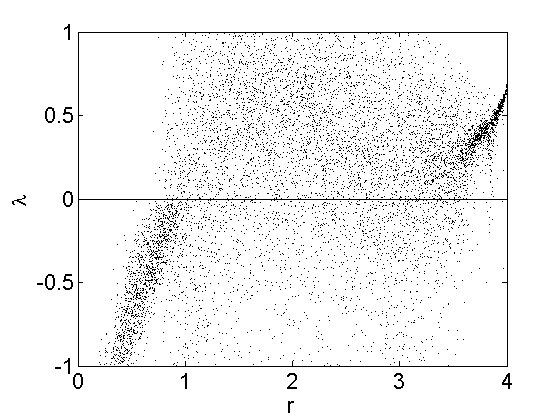
\includegraphics[scale=0.65]{figs/rlog_lyap_all.png}
% 	\end{center}
% \end{figure} 
An unexpected result of the simulation is the presence of the stable
periodic orbits in the right side of the bifurcation diagram
(Figure~\ref{fig:rlogbif_low} and
Figure~\ref{fig:rlogbif}). Specifically, this region occurs between $r
\in [3,4]$, and is most dominantly featured for the bifurcation diagram with $L=0.1$. In the
deterministic case (Figure~\ref{fig:bif}), this region was previously
unstable. Examining the Lyapunov exponent of the randomized logistic
map gives some insight on whether the map is possibly chaotic. The
exponent of the deterministic map is on the top left of Figure~\ref{fig:rloglyap2},
and we see there is a point in $r$ where stable behavior transitions
to chaotic behavior (just under $r=3.6$). In the randomized case, the
delimination is unclear. However one feature of the deterministic
diagram seems to be preserved, and that is the negative spike around
$r=3.8$.

A histogram describing the average fraction of observed period $p$
orbits is shown in Figure~\ref{fig:rloghist}. The histogram implies
that the most commonly observed stable orbit is period 2, and the
distribution of periodic orbits may follow the exponential distribution.

\begin{figure}[H]\linespread{1}
\caption[Random logistic map bifurcation diagram, low resolution]{A
  low-resolution bifurcation diagram of the random
logistic map, where $r \in [0,4]$, $\Delta r = 0.009$ (stepsize
between each discretized value of $r$), $N=100$, the
number of initial conditions $N_{x_0}=100$, and $L=0.1$. Results from
45,000 simulations are plotted. The colorbar to the right shows the
color for each period. Orbits up to period 52 were checked.}\label{fig:rlogbif_low}
	\begin{center}
          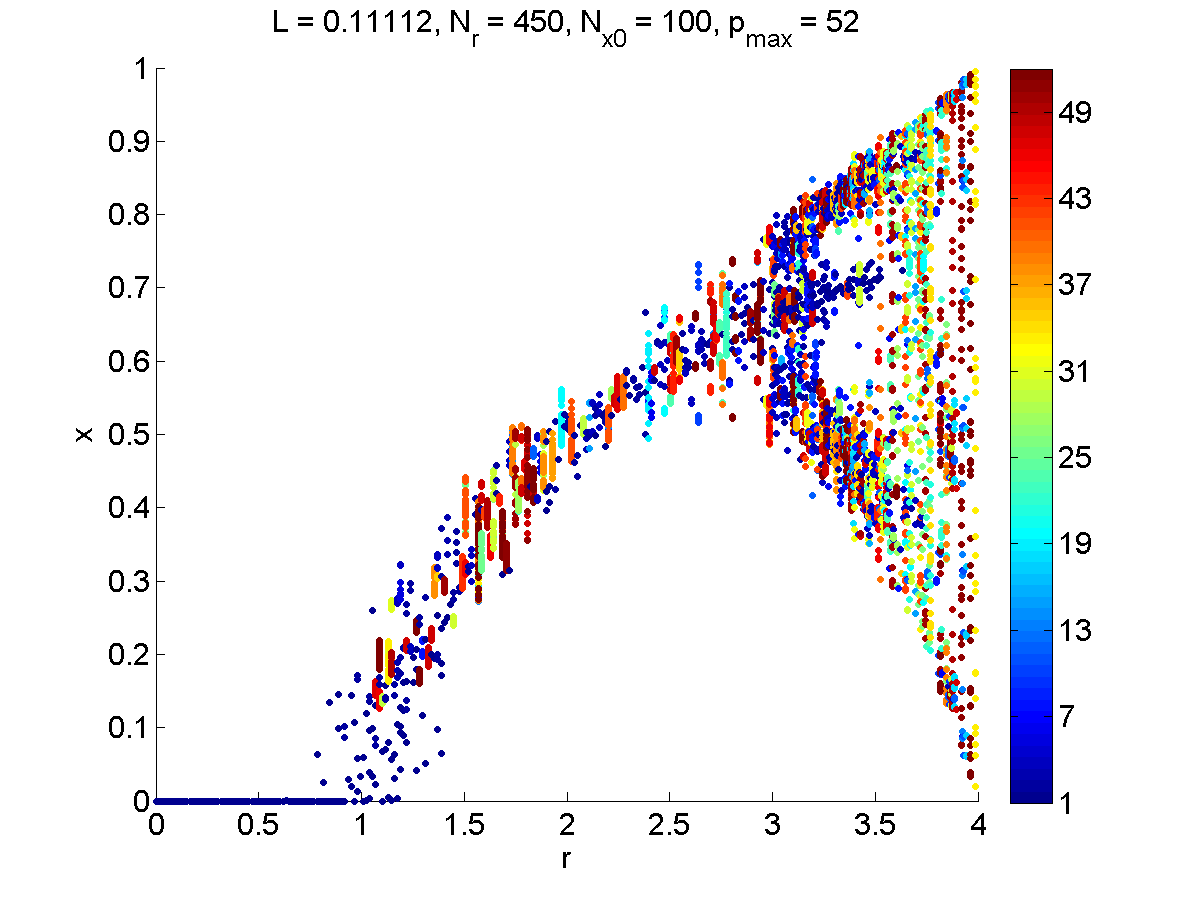
\includegraphics[scale=0.48]{figs/rlog_bif_L_01_low.png}
	\end{center}
\end{figure}
\begin{figure}[H]\linespread{1}
\caption[Average number of period $p$ orbits for the random logistic
map]{Average number of period $p$ orbits for the random logistic
map, where $r =3.2$,$L=0.1$,$N=100$, and $\sigma = 0.0061$. Results from 2000
simulations of these parameters are plotted. The error bars indicate
the standard error of the calculation of the mean for 2000 samples.}\label{fig:rloghist}
	\begin{center}
          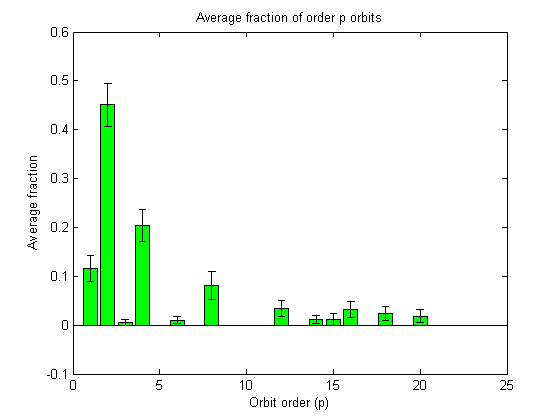
\includegraphics[scale=0.65]{figs/rlog_hist_r32_L01.png}
	\end{center}
\end{figure}

\begin{figure}[H]\linespread{1}
\caption[Bifurcation diagram of the random logistic map, high resolution]{Bifurcation diagram of the random
logistic map, where $r \in [0,4]$, $\Delta r = 0.002$, $N=100$, the
number of initial conditions $N_{x_0}=1000$, and $L\in
\{0.1,0.2,0.4,0.6,0.8,0.9\}$. Plots are read left to right, and top to
bottom. Results from 1.8 million simulations are plotted. The colorbar
to the right shows the color for each period. Orbits up to period 256 were checked.}\label{fig:rlogbif}
	\begin{center}
		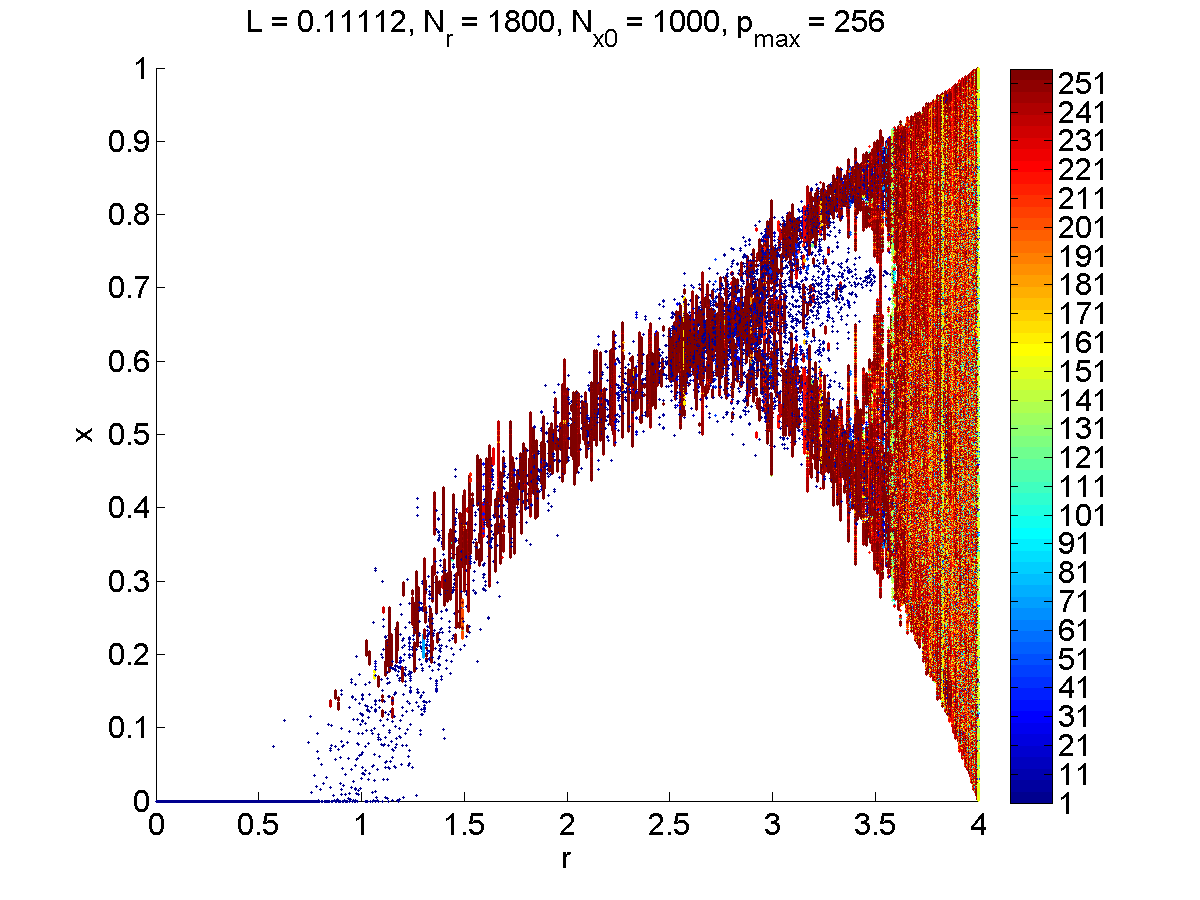
\includegraphics[width=.5\textwidth]{figs/rlog_bif_L_01.png}\hfill
		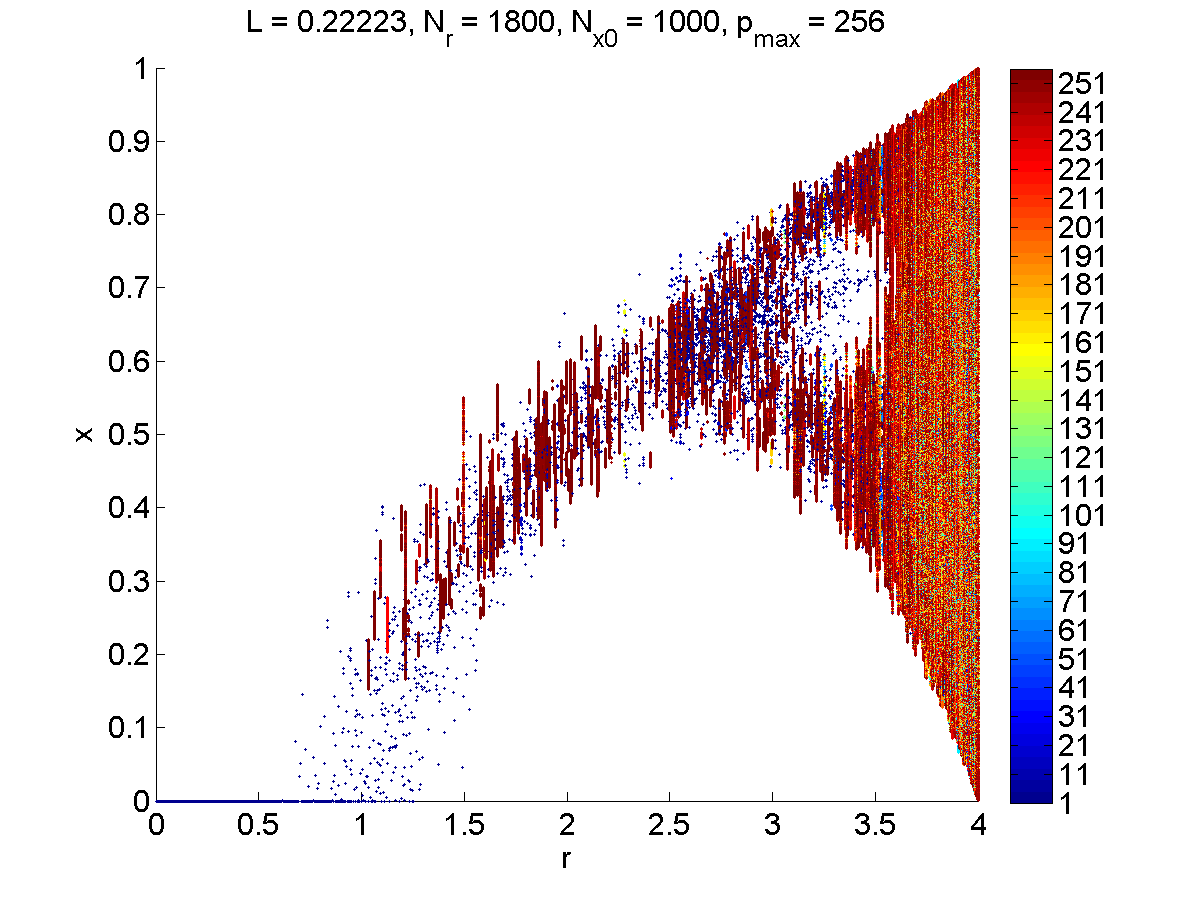
\includegraphics[width=.5\textwidth]{figs/rlog_bif_L_02.png}\\
		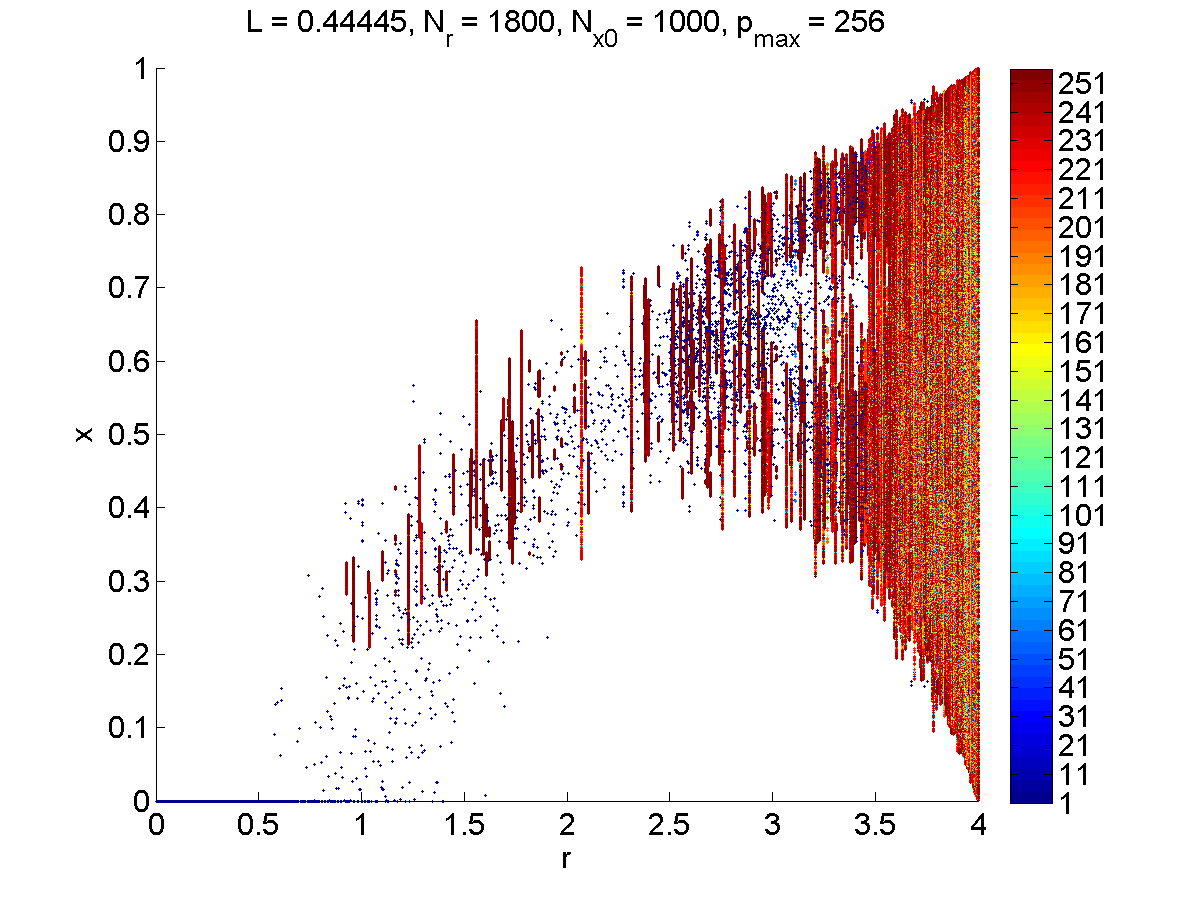
\includegraphics[width=.5\textwidth]{figs/rlog_bif_L_04.png}\hfill
		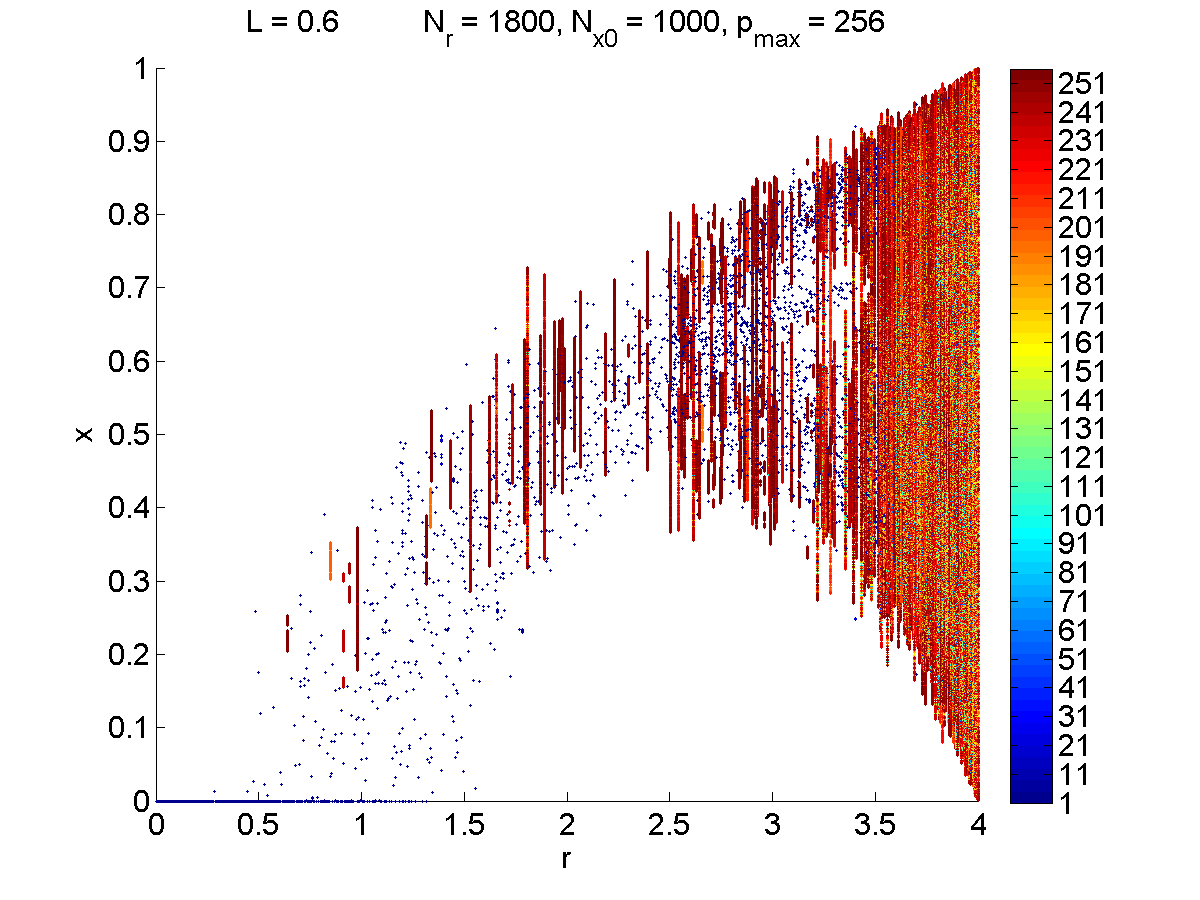
\includegraphics[width=.5\textwidth]{figs/rlog_bif_L_06.png}\\
		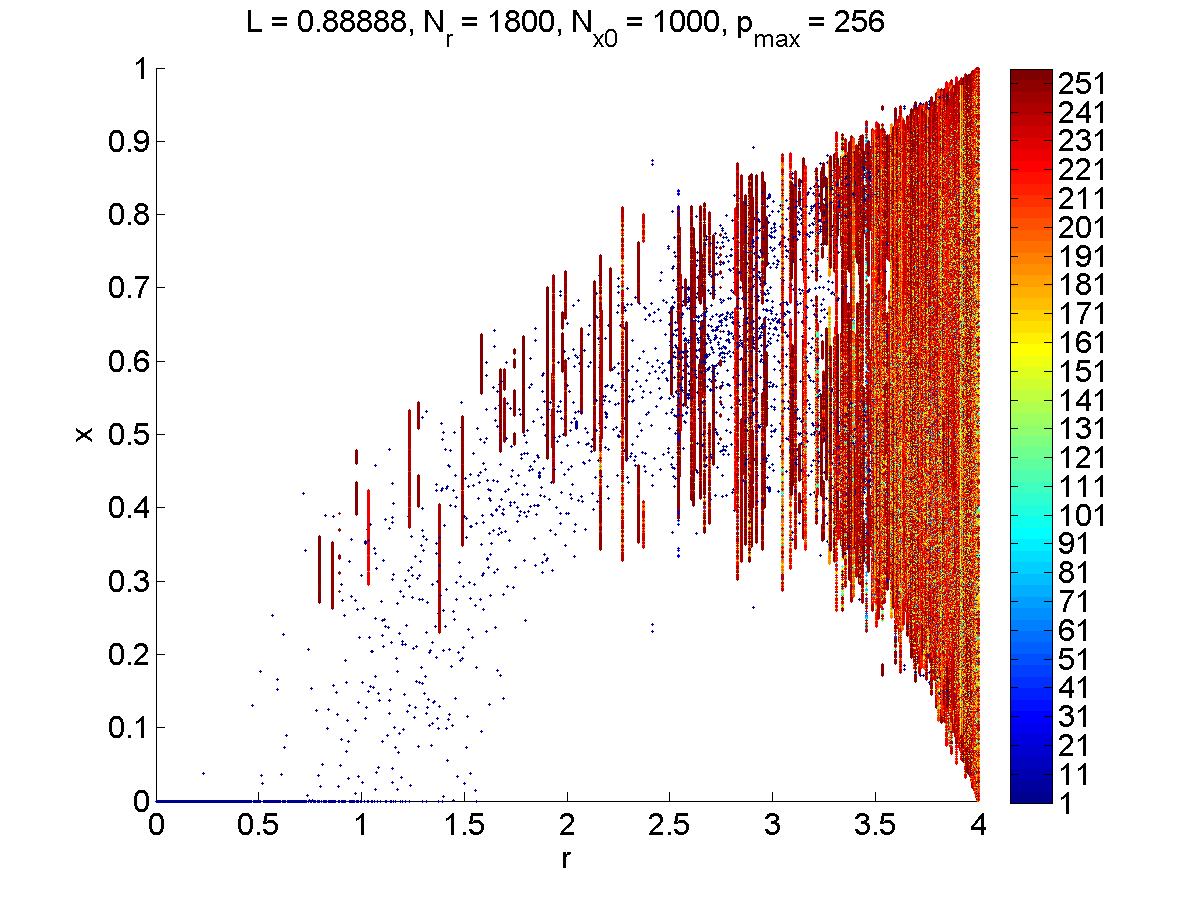
\includegraphics[width=.5\textwidth]{figs/rlog_bif_L_08.png}\hfill
		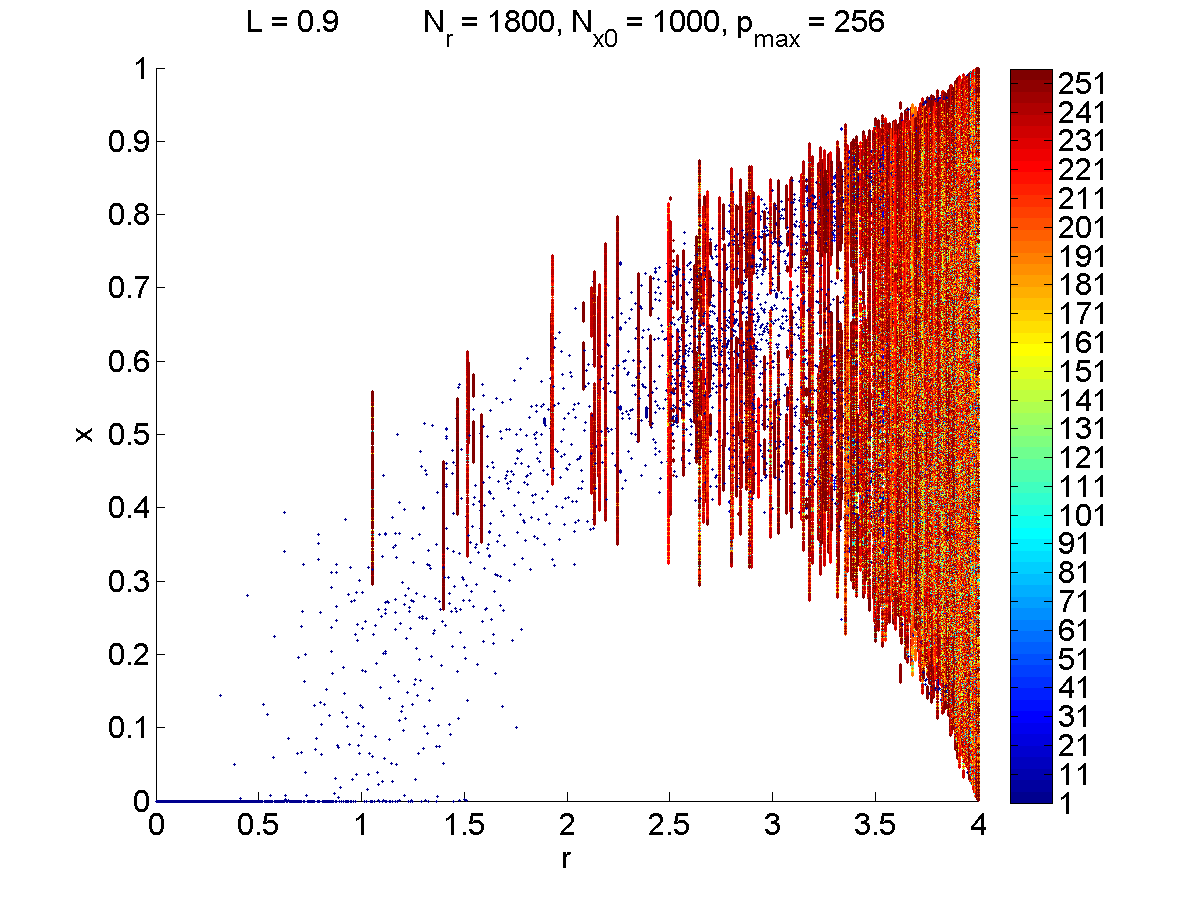
\includegraphics[width=.5\textwidth]{figs/rlog_bif_L_09.png}\\
	\end{center}
\end{figure}

\begin{figure}[H]\linespread{1}
\caption[Bifurcation diagram of the random logistic map, zoomed
in]{A zoomed in view of Figure~\ref{fig:rlogbif}, where $r \in
  [3,4]$, $\Delta r = 0.001$, $N=100$, the number of initial
  conditions $N_{x_0}=1000$, and $L\in \{0.1,0.2,0.4,0.6,0.8,0.9\}$.}
	\begin{center}
		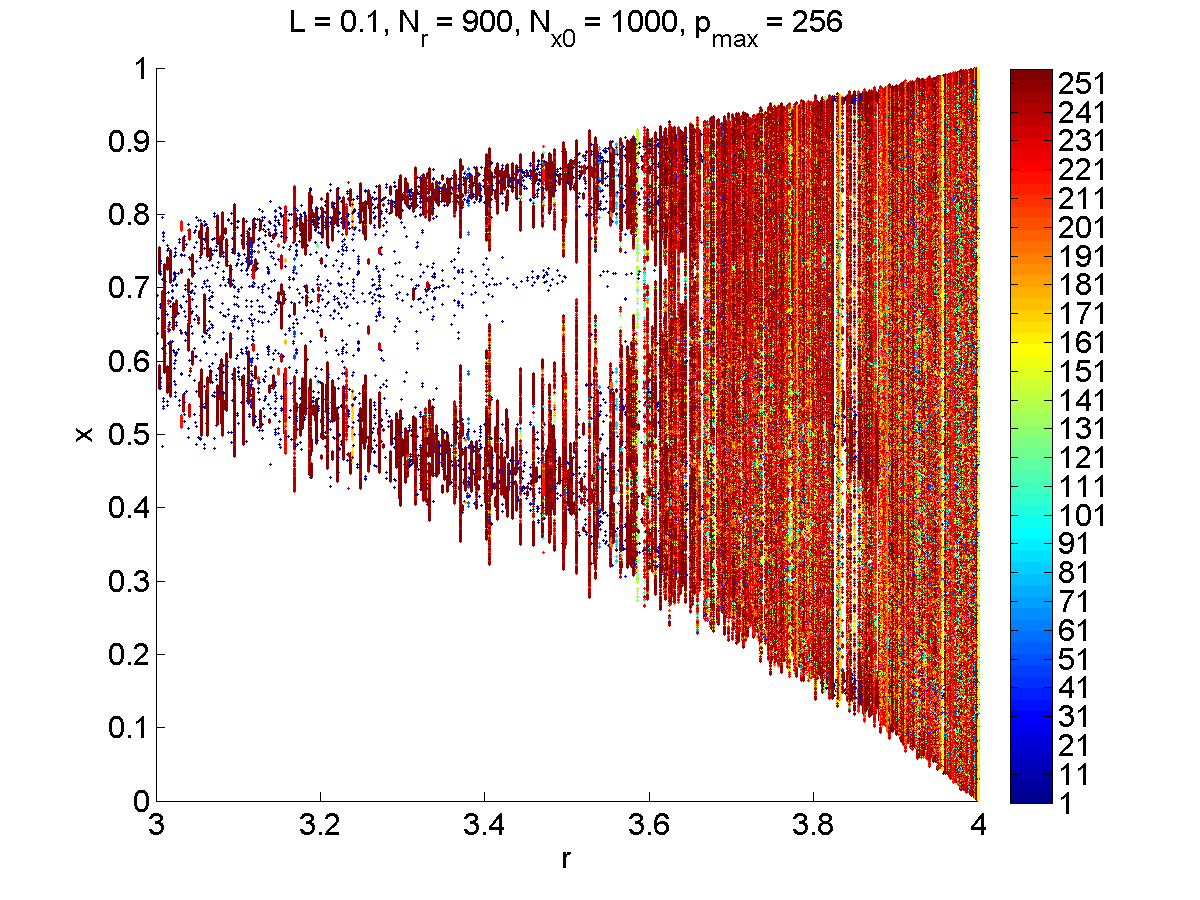
\includegraphics[width=.5\textwidth]{figs/rlog_bif_zoom_L_01.png}\hfill
		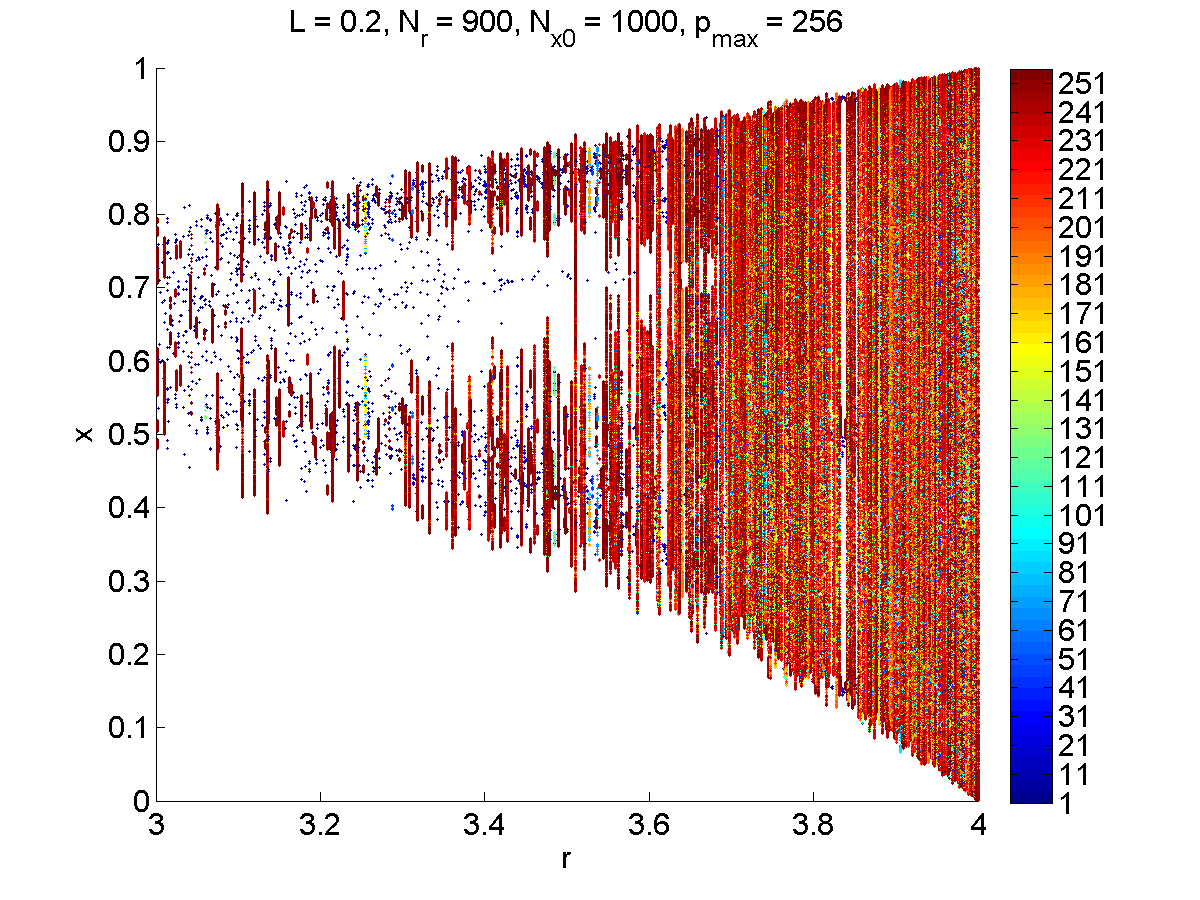
\includegraphics[width=.5\textwidth]{figs/rlog_bif_zoom_L_02.png}\\
		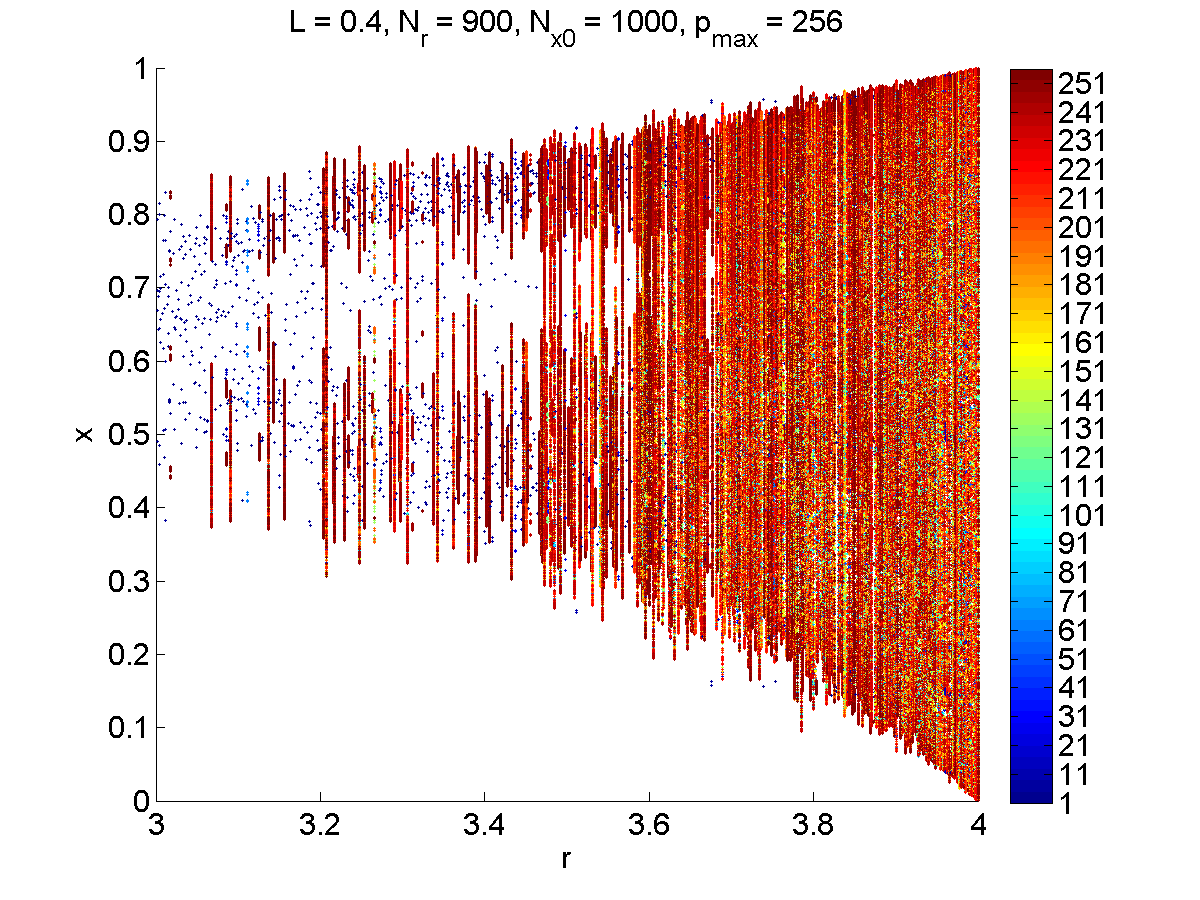
\includegraphics[width=.5\textwidth]{figs/rlog_bif_zoom_L_04.png}\hfill
		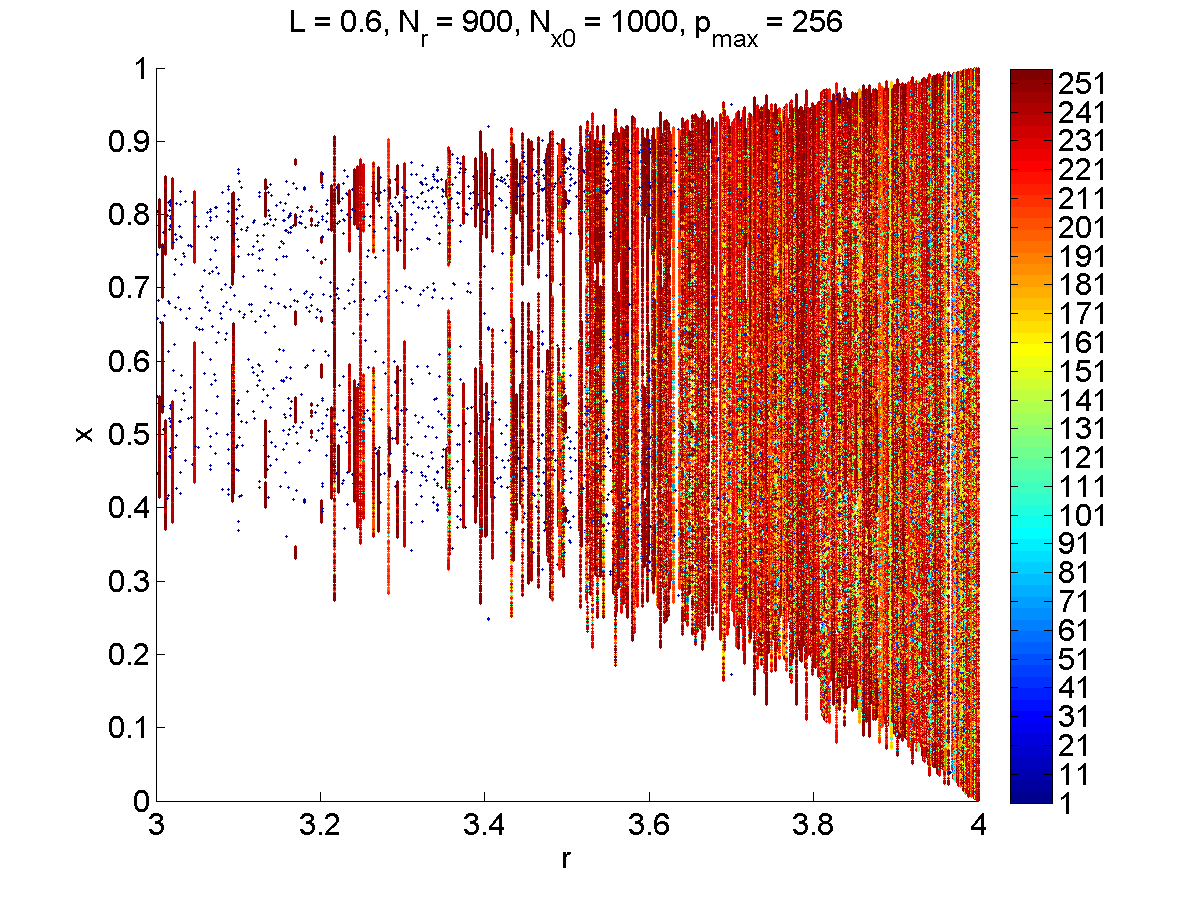
\includegraphics[width=.5\textwidth]{figs/rlog_bif_zoom_L_06.png}\\
		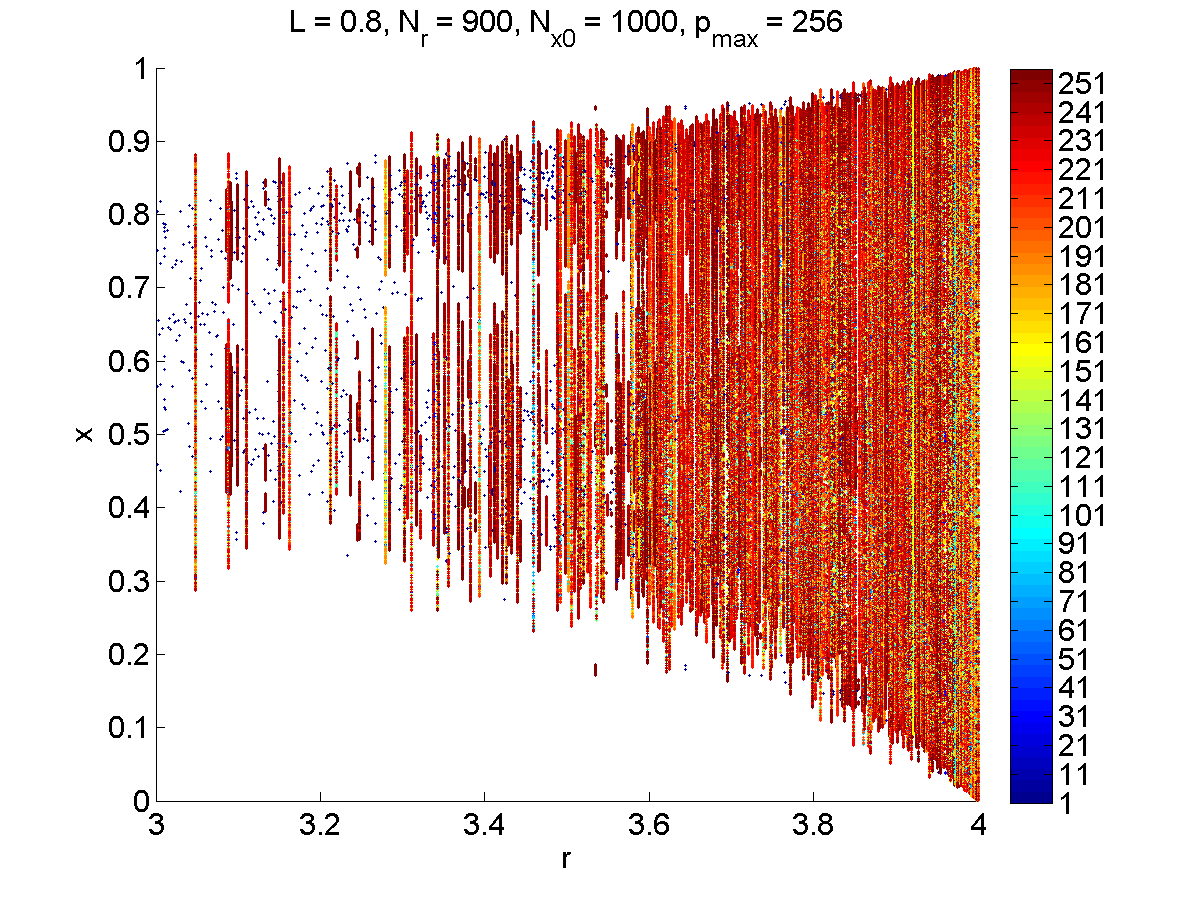
\includegraphics[width=.5\textwidth]{figs/rlog_bif_zoom_L_08.png}\hfill
		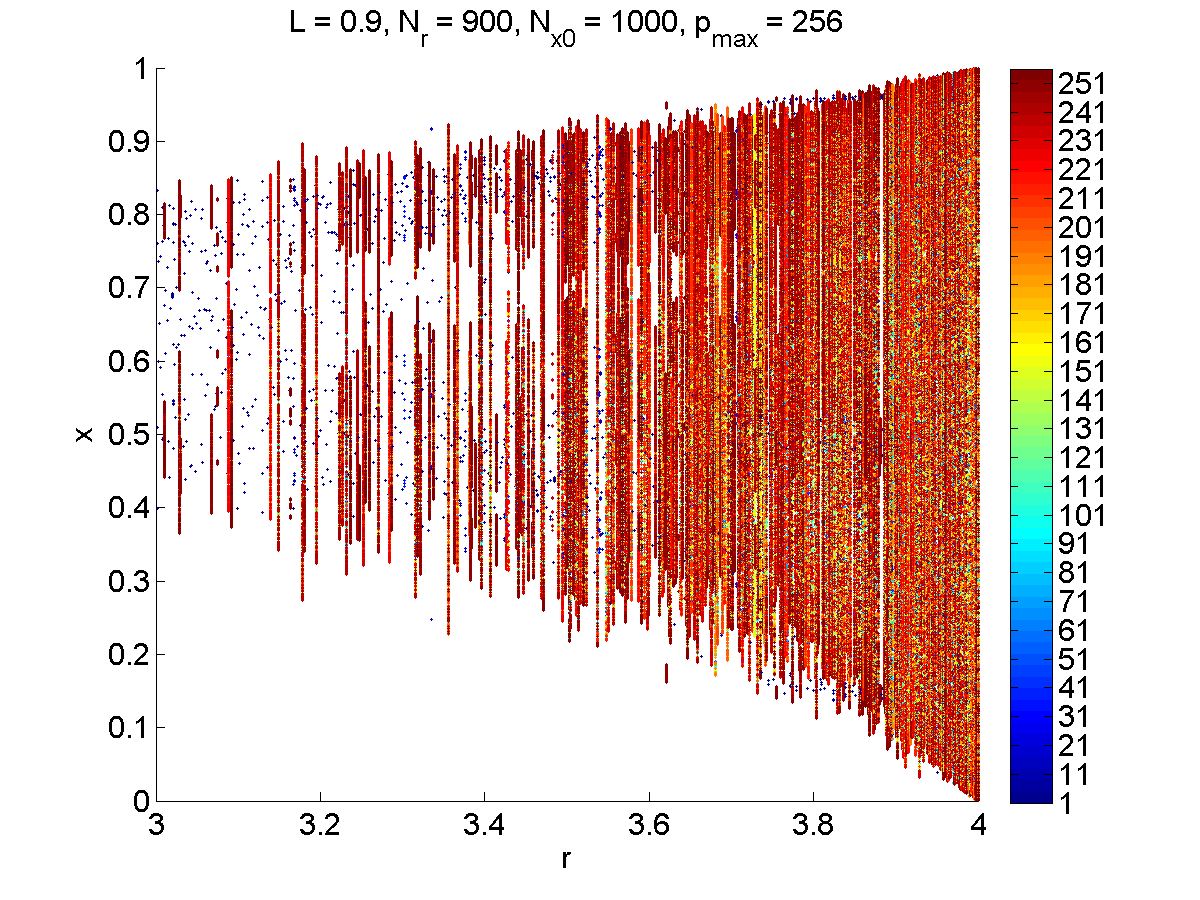
\includegraphics[width=.5\textwidth]{figs/rlog_bif_zoom_L_09.png}\\
	\end{center}
\end{figure}
\begin{figure}[!h]
\caption[Lyapunov exponent in the random logistic map compared to the
deterministic map]{The Lyapunov exponent for the deterministic
  logistic map (top left) is compared
  to the Lyapunov exponent of the random logistic map for $L \in \{0.05,0.1,0.5,0.7,0.9\}$, where $x_0=0.7$ for $r \in [3,4]$. The number of exponents computed over
  [3,4] was $N_\lambda=10,000$. Plots are read left to right, and top
  to bottom. }\label{fig:rloglyap2}
\centering
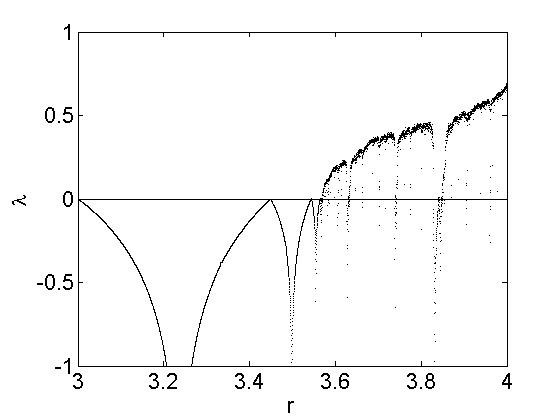
\includegraphics[width=.5\textwidth]{figs/det_log_lyap.png}\hfill
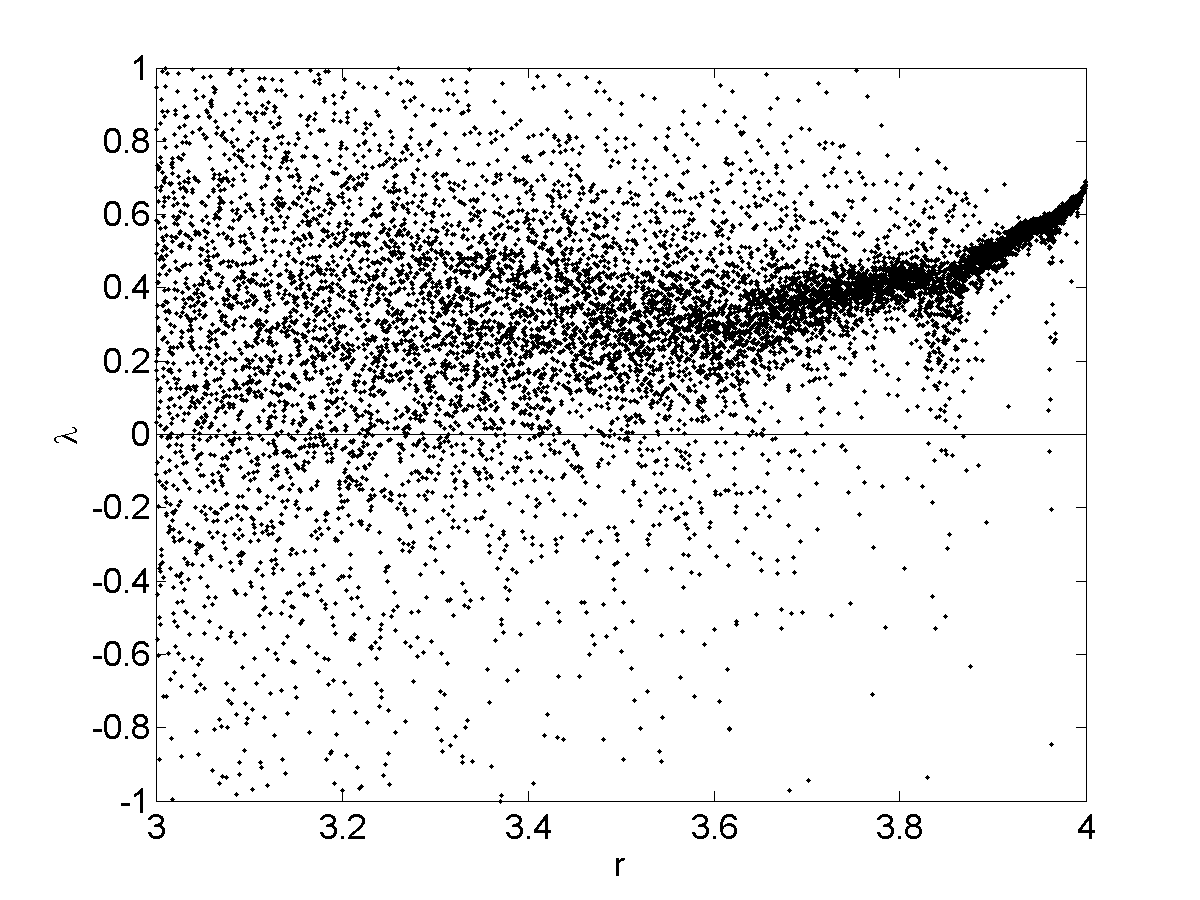
\includegraphics[width=.5\textwidth]{figs/rlog_lyap_L_005.png}\\
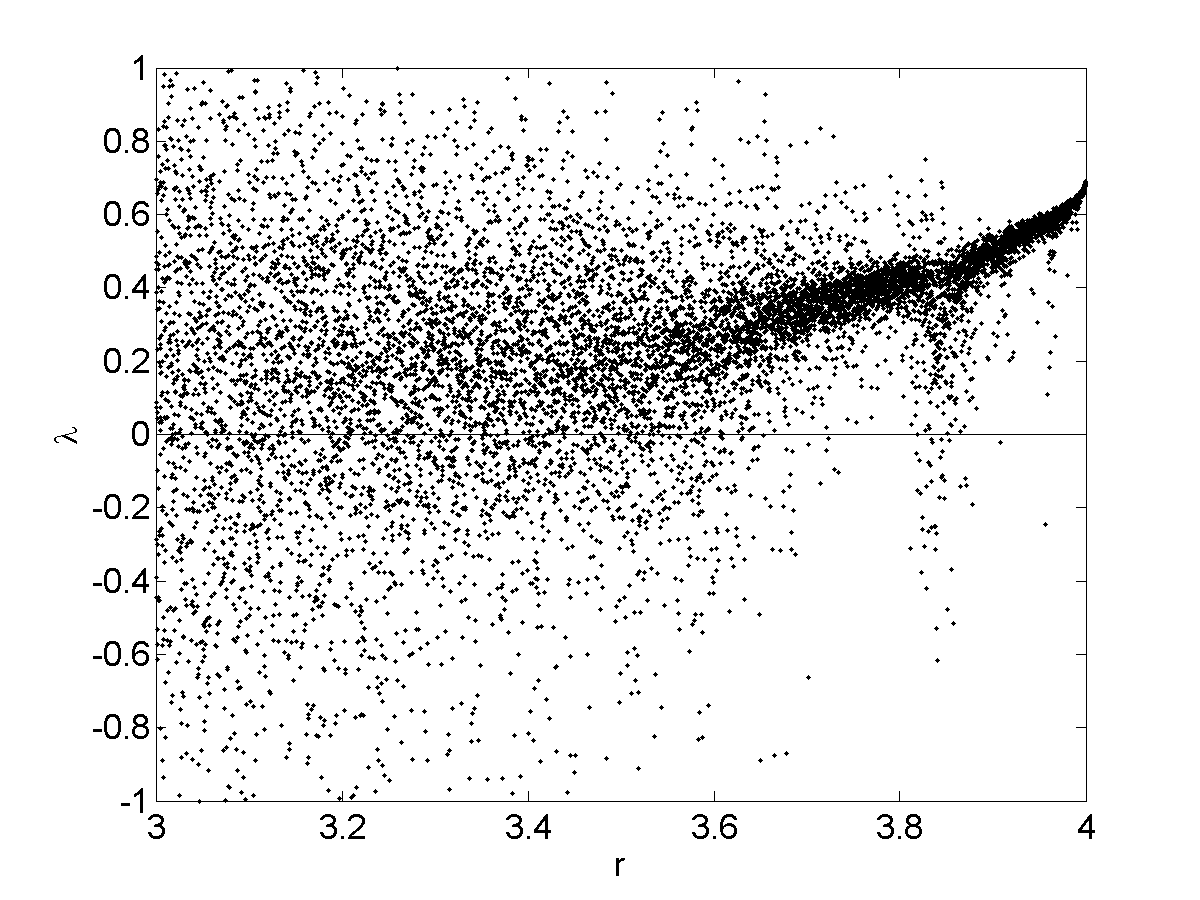
\includegraphics[width=.5\textwidth]{figs/rlog_lyap_L_01.png}\hfill
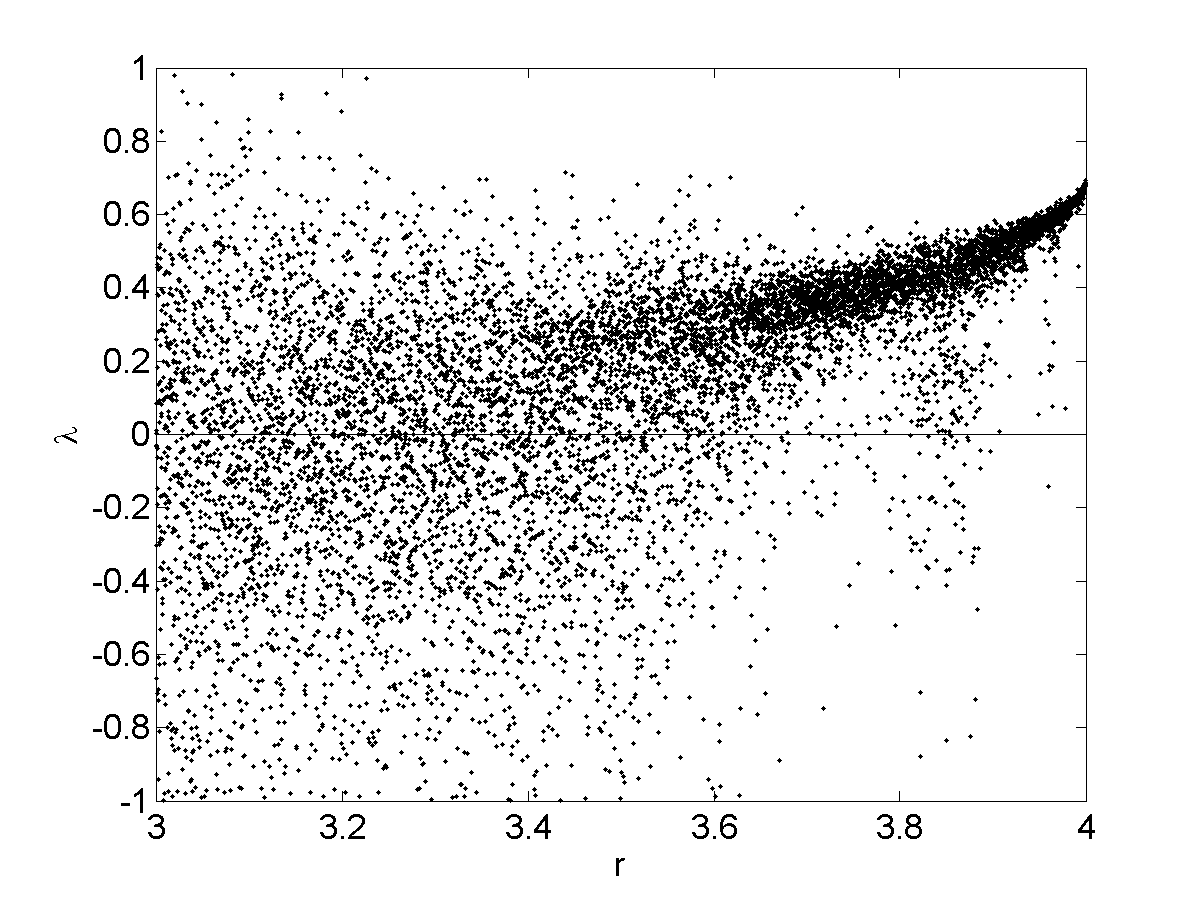
\includegraphics[width=.5\textwidth]{figs/rlog_lyap_L_05.png}\\
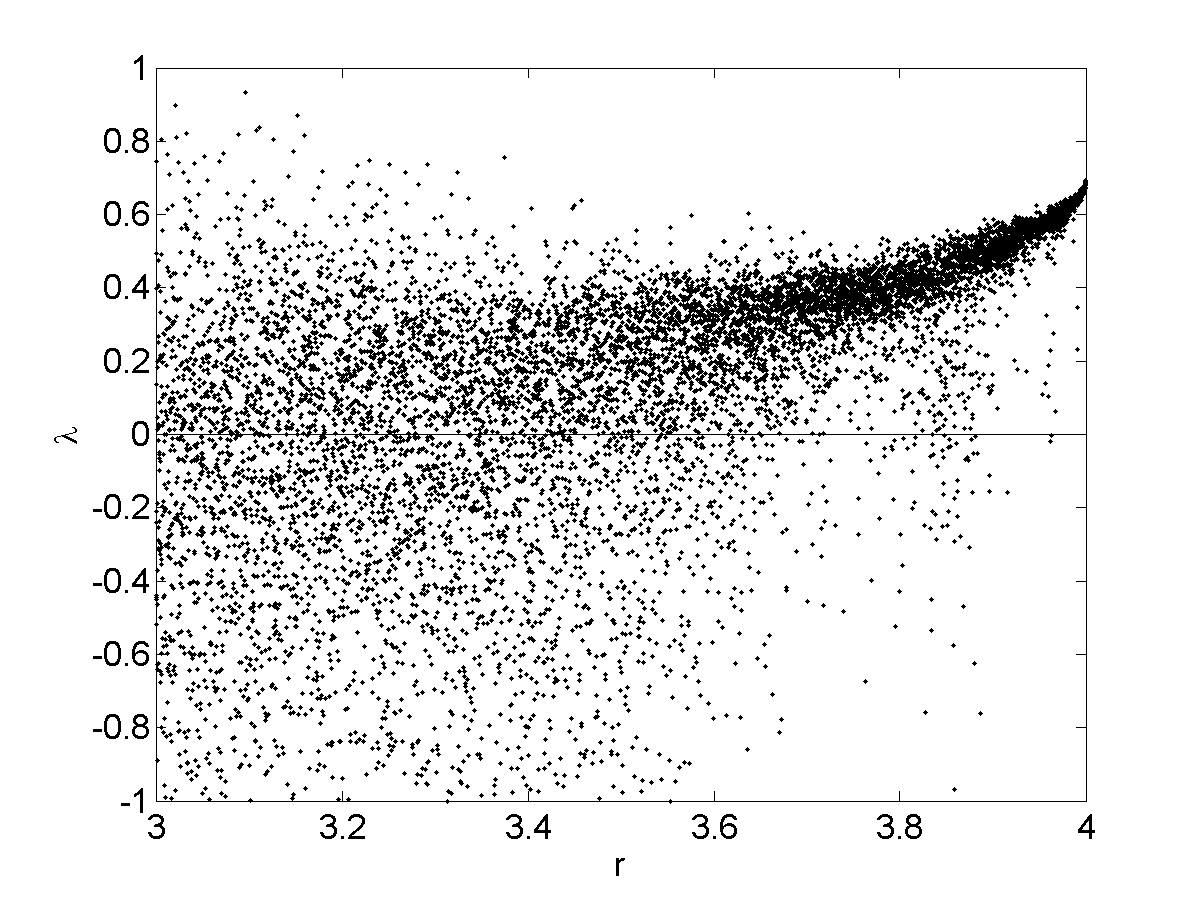
\includegraphics[width=.5\textwidth]{figs/rlog_lyap_L_07.png}\hfill
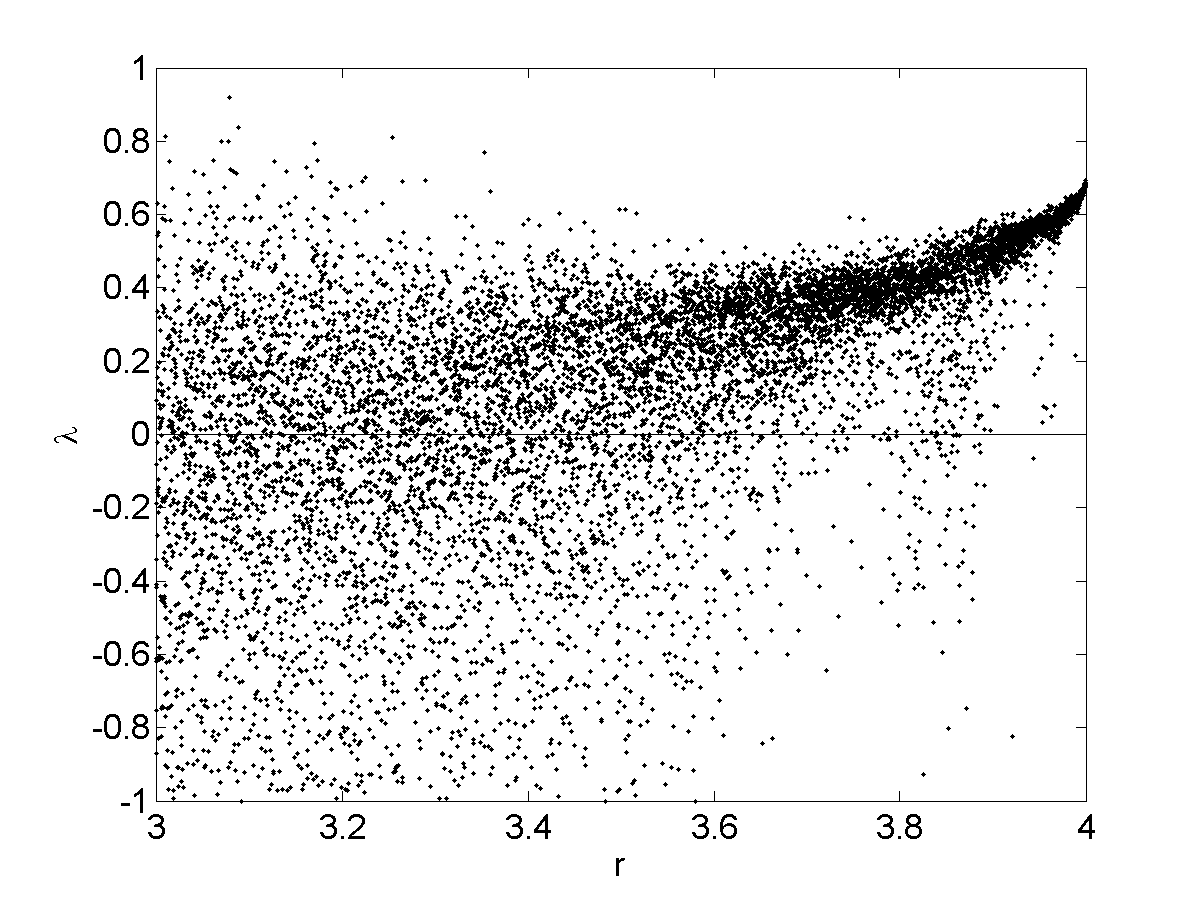
\includegraphics[width=.5\textwidth]{figs/rlog_lyap_L_09.png}\\
\end{figure}

\section{Implementation of Randomness in the Circle Map}
The randomized circle map has a set of Arnold Tongues (Figure~\ref{fig:rcirctongues_u} and
Figure~\ref{fig:rcirctongues_n}) that has almost no similarity to the deterministic
case, for both the cases where the randomness is based on the uniform
and Gaussian distributions. For low values of $L$, we have lost the
shape of the tongues, and the diagram becomes asymmetrical. For larger
values of $L$, the distinctive tongues and the overall symmetry is
recovered. The randomness appears to have an overall destabilizing
effect on the dynamics of the map.

A comparison of the Lyapunov exponent of the deterministic and random
case (Figure~\ref{fig:rcirclyap_n}) partially confirms the idea that
the noise is destabilizing; nearly no features of the deterministic
graph are preserved, and the high density of positive values indicates
chaotic behavior. A similarity between the simulations involving the uniform and normal
distributions is that they both produced plots of Lyapunov exponents that seem to have a
high density of exponents in the lower right corner
(Figure~\ref{fig:rcirclyap_u} and Figure~\ref{fig:rcirclyap_n}), but
only for the case where one varies $\omega$ and fixes $k$ to be constant.

Further, a plot of the average number of orbits
(Figure~\ref{fig:avgcircorbs}) for the random process based on the
uniform distribution shows the largest number of orbits over 1000
simulations is period 1. The parameters tested in this simulation were
for $k=1, \omega=0.1$, which corresponds to a stable period 1 region
in the bifurcation diagram (middle left in
Figure~\ref{fig:rcirctongues_u}). This demonstrates the presence of
stable high-period orbits, where previously there were only
stable period 1 orbits in the deterministic map.

% In Figure~\ref{fig:rcirc_bifw_u}, it appears that as $\omega$ is
% varied over $[0,1]$ (for fixed $k=1$), the distribution of stable
% orbits follows the line $x=\omega$. However, closer examination of the
% solutions of (\ref{randcirc}) demonstrate
% \begin{align*}
% \begin{split}
% \omega &= \frac{k}{2\pi}\sin(2\pi x)\\
% x &= \frac{1}{2\pi}\arcsin\left(\frac{2\pi \omega}{k}\right).
% \end{split}
% \end{align*}

\subsection{Uniform Distribution}
\begin{figure}[H]\linespread{1}  
\caption[The Arnold tongues for the random circle map, uniform distribution]{The Arnold
  tongues for $k\in [0,1.5]$, $\Delta k = 0.0015$, $\omega \in [0,1]$,
  $\Delta \omega = 0.001$, $\alpha = 10^{-5}$, $\hat{\xi}_n\sim Unif(-M_n,M_n)$ and $L_j \in
  \{10^{-6},0.05,0.1,0.3,0.5,0.9\}$. Plots are ordered left to right, and top to bottom. The colorbar
to the right demonstrates the period and corresponding color.}\label{fig:rcirctongues_u}
\centering
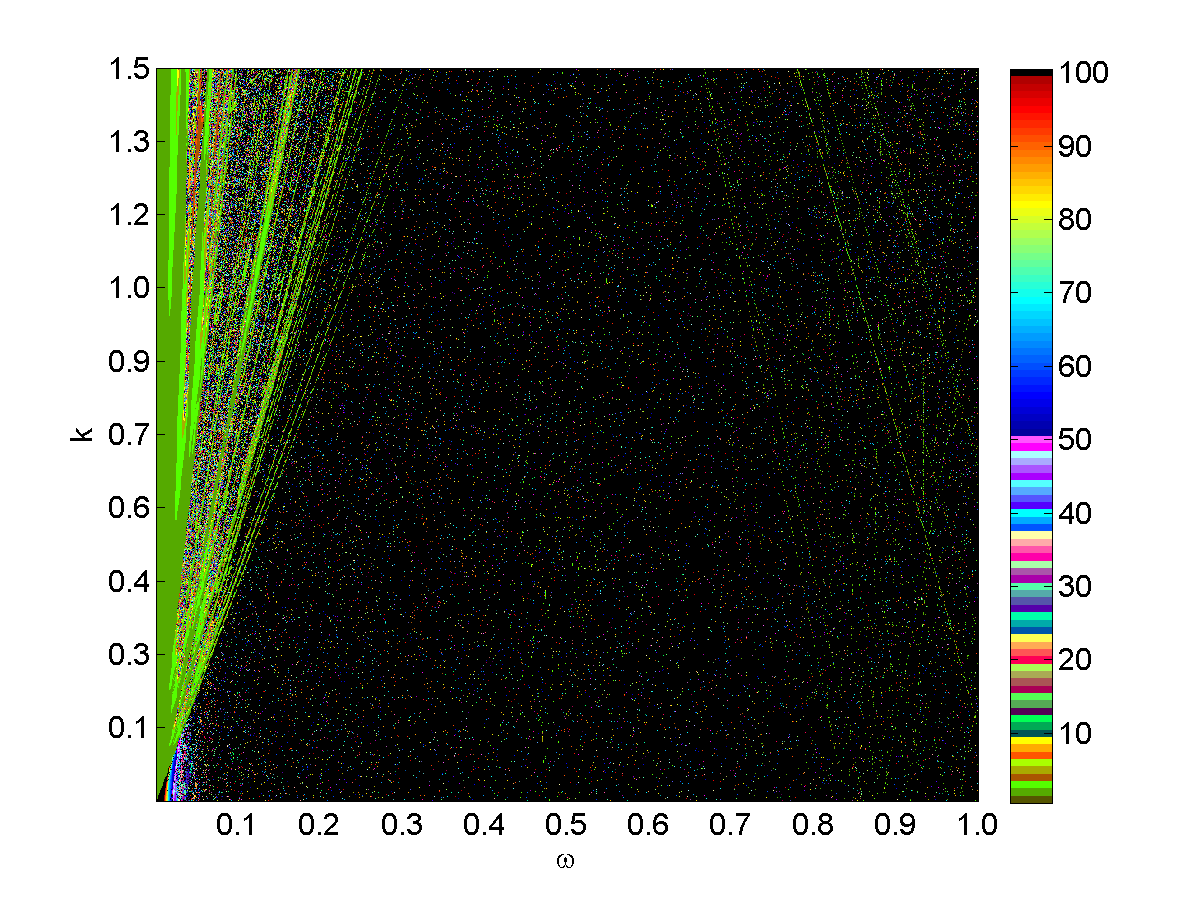
\includegraphics[width=.5\textwidth]{figs/tongues_1000_L_1e-05.png}\hfill
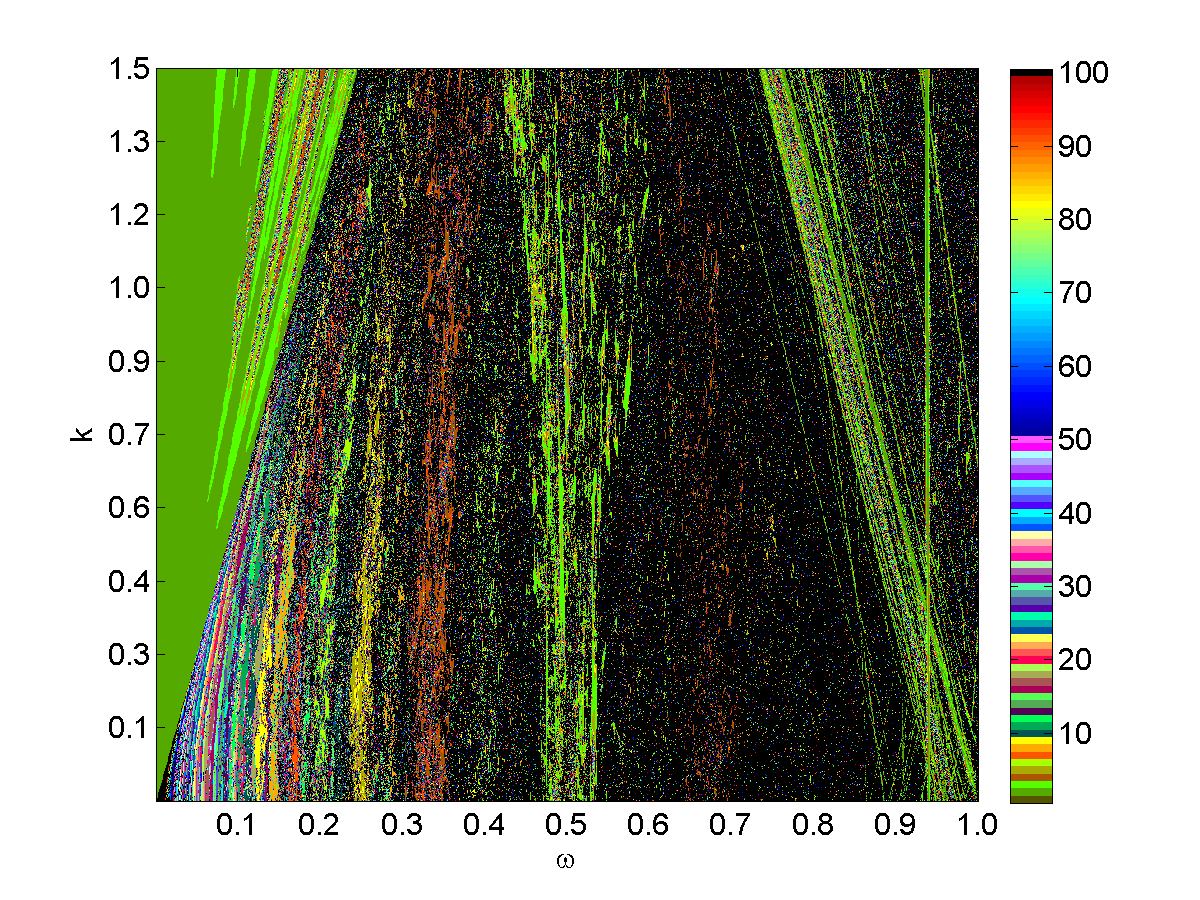
\includegraphics[width=.5\textwidth]{figs/tongues_1000_L_005.png}\\
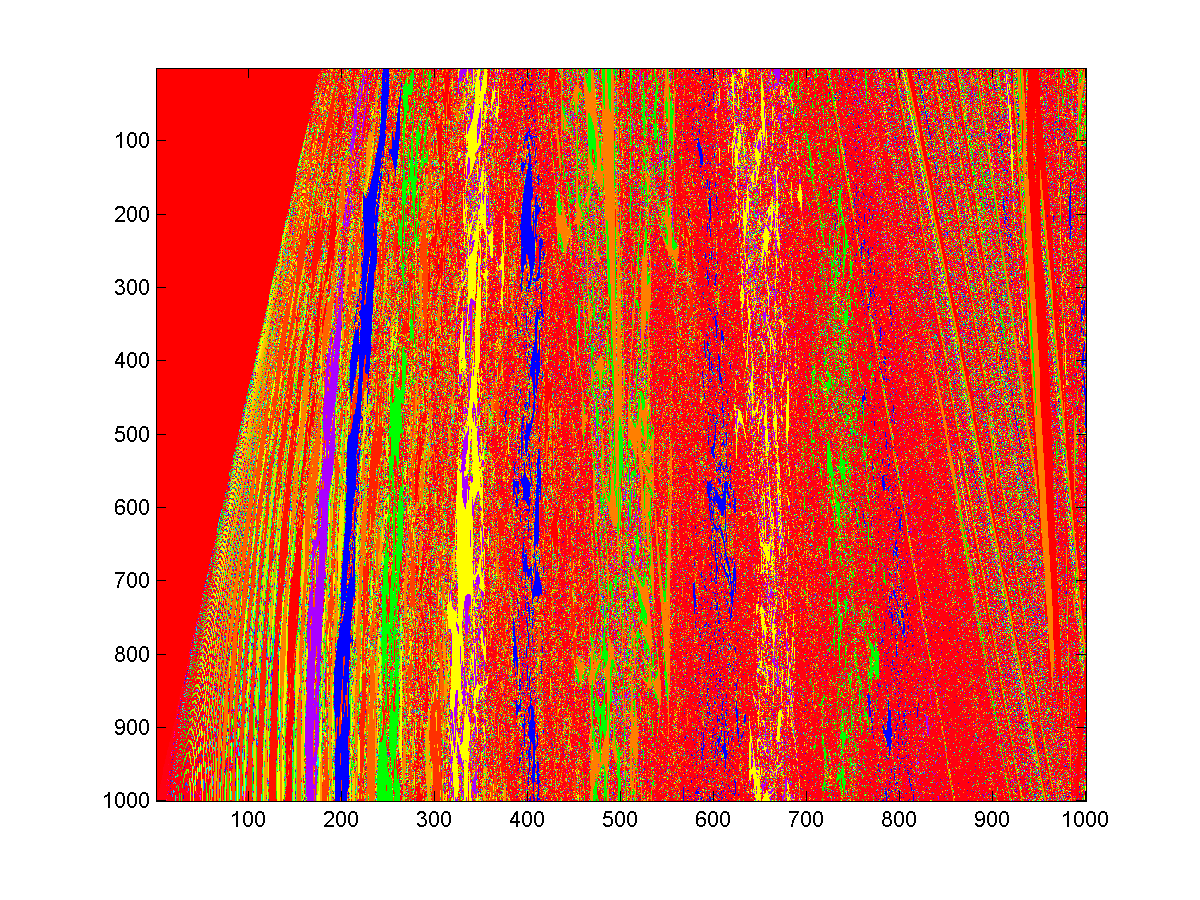
\includegraphics[width=.5\textwidth]{figs/tongues_1000_L_01.png}\hfill
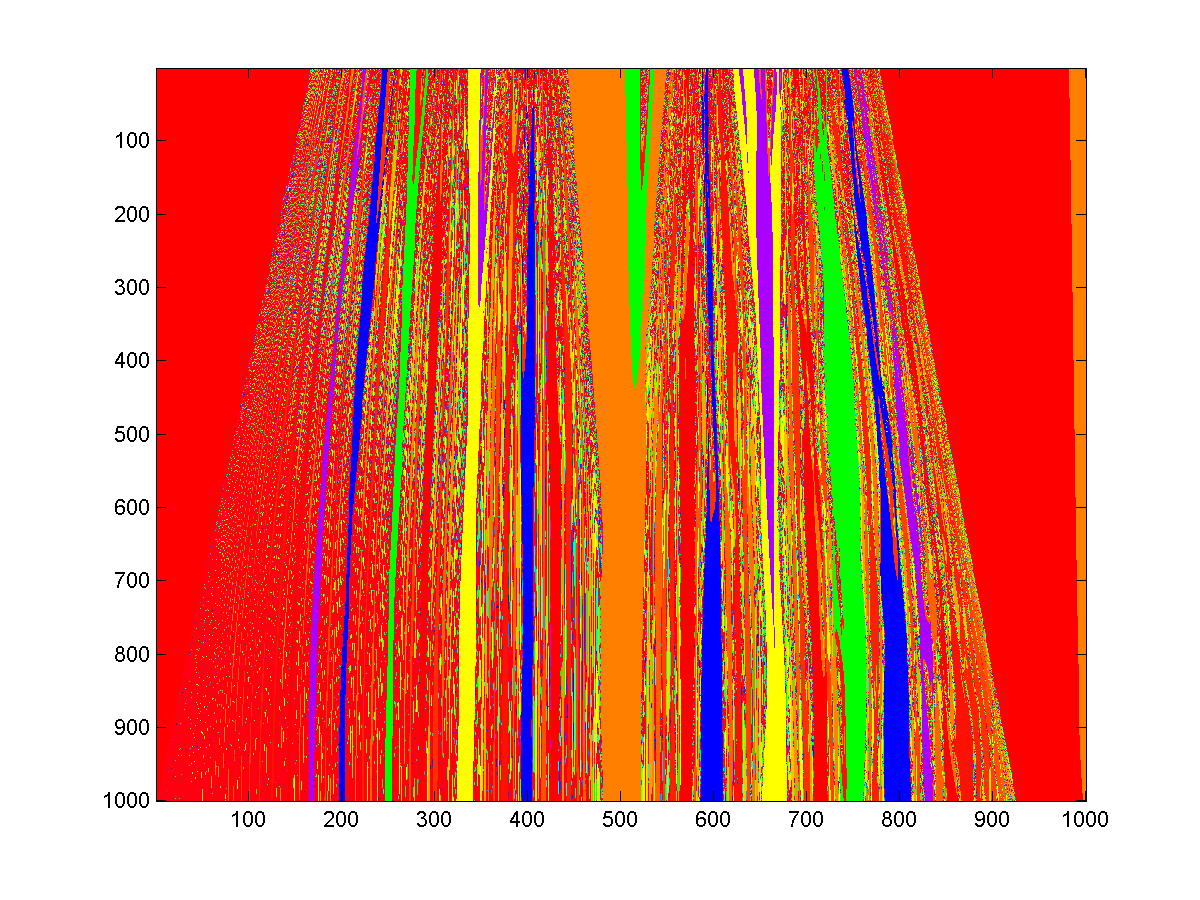
\includegraphics[width=.5\textwidth]{figs/tongues_1000_L_03.png}\\
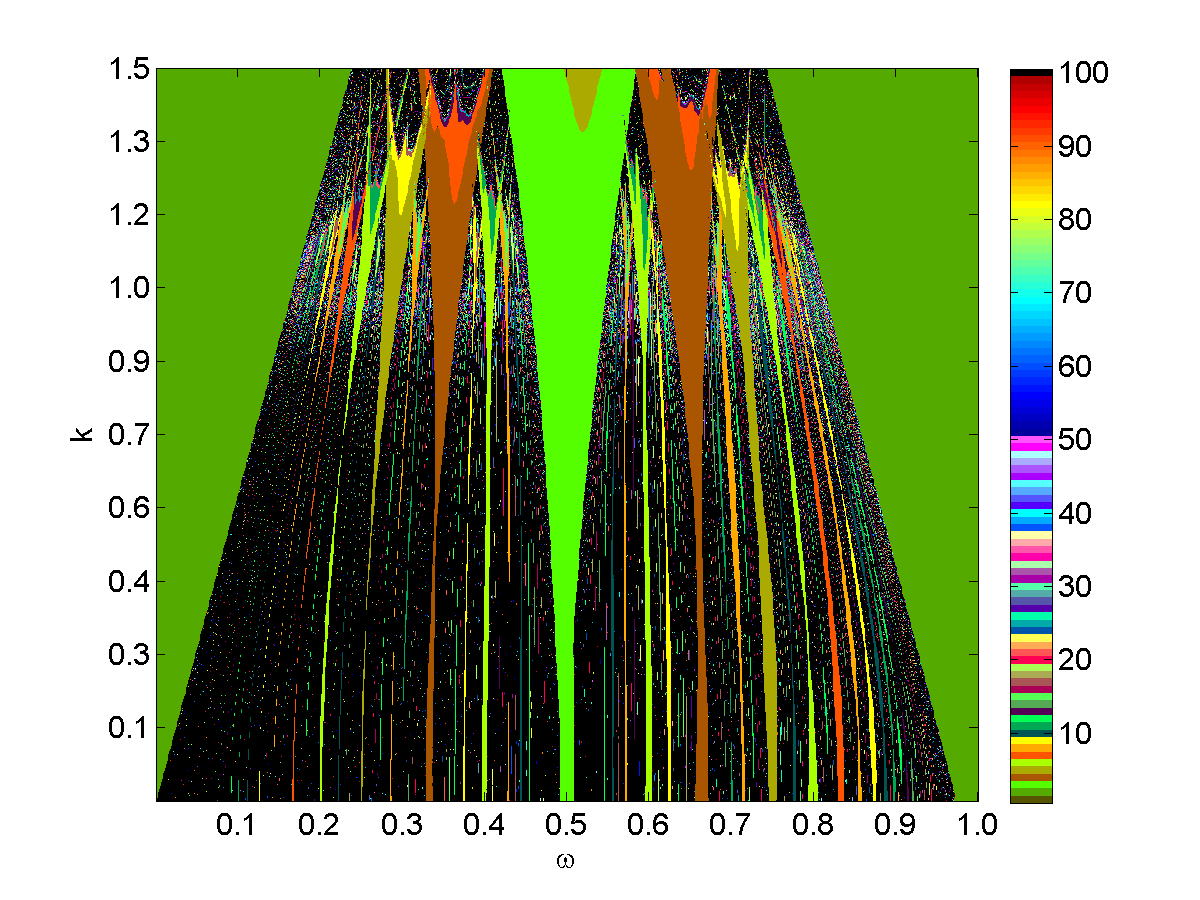
\includegraphics[width=.5\textwidth]{figs/tongues_1000_L_05.png}\hfill
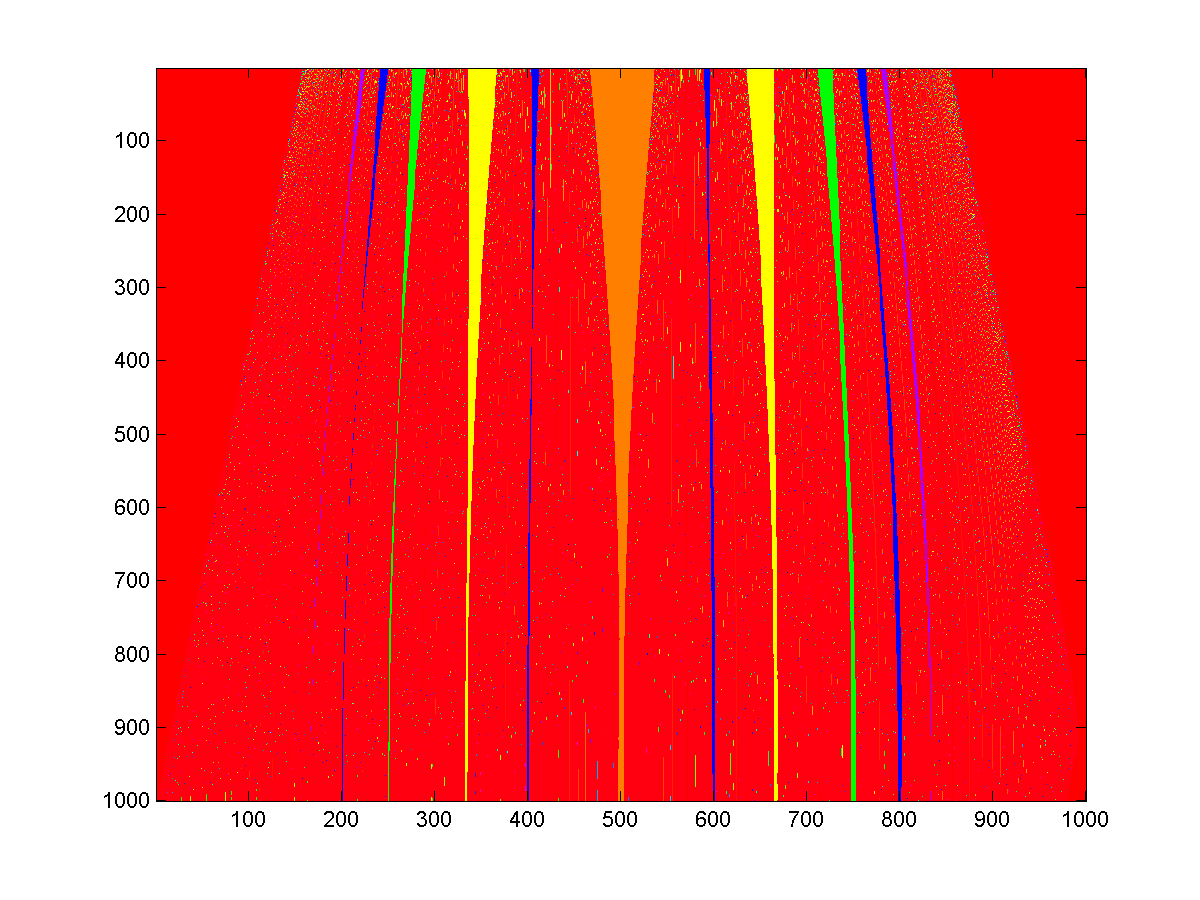
\includegraphics[width=.5\textwidth]{figs/tongues_1000_L_09.png}\\
\end{figure}

\begin{figure}[!h]
\caption[Lyapunov exponent in the random circle map (uniform distribution) compared to the
deterministic map, varying $\omega$]{The Lyapunov exponent for the deterministic
  circle map (top left) is compared
  to the Lyapunov exponent of the random circle map for $L \in
  \{0.05,0.1,0.3,0.5,0.9\}$, where $x_0=0.7$, $k=2$,$\alpha =
  10^{-5}$, and $\hat{\xi}_n\sim
  Unif(-M_n,M_n)$ for $\omega \in [0,1]$. The number of exponents computed was $N_\lambda=10,000$. Plots are read left to right, and top to bottom. }\label{fig:rcirclyap_u}
\centering
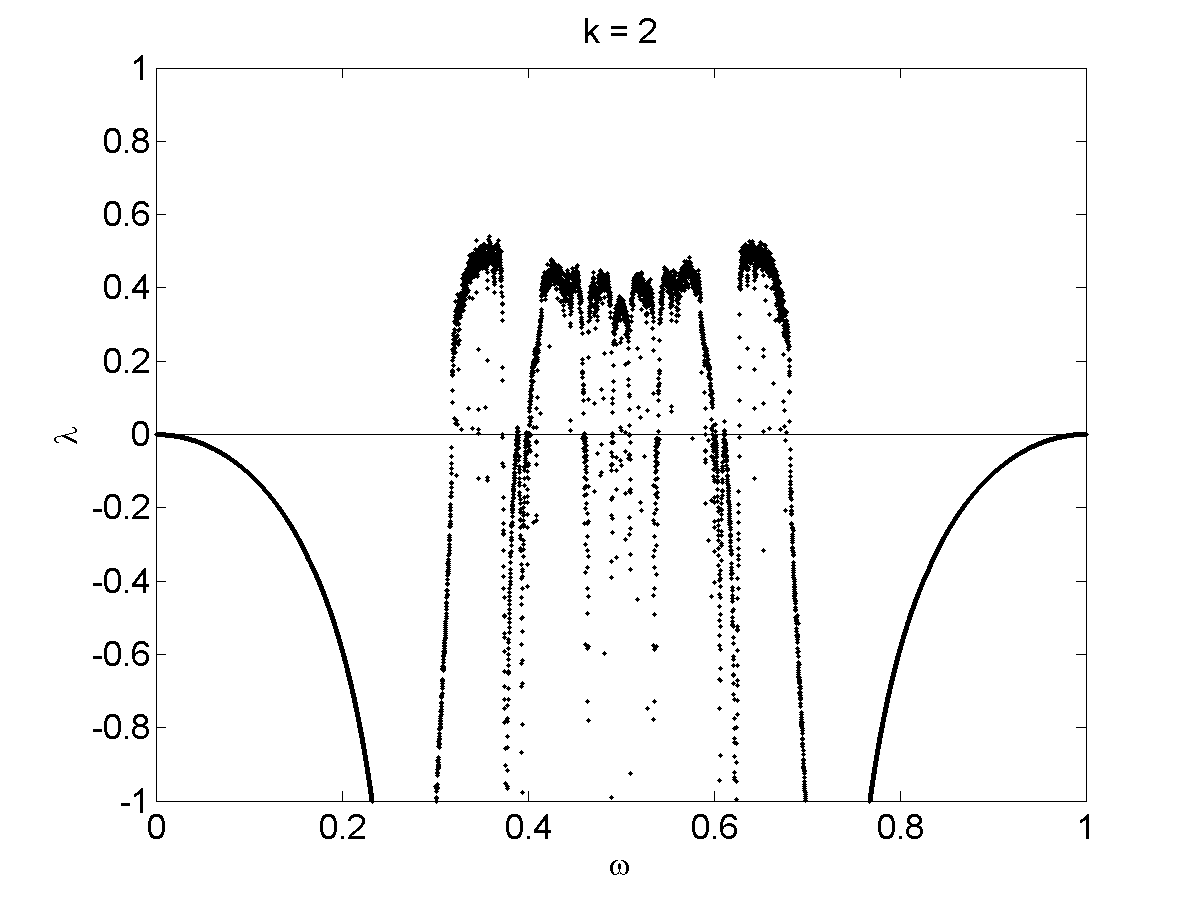
\includegraphics[width=.5\textwidth]{figs/detcirc_lyap_10000_k_2_w.png}\hfill
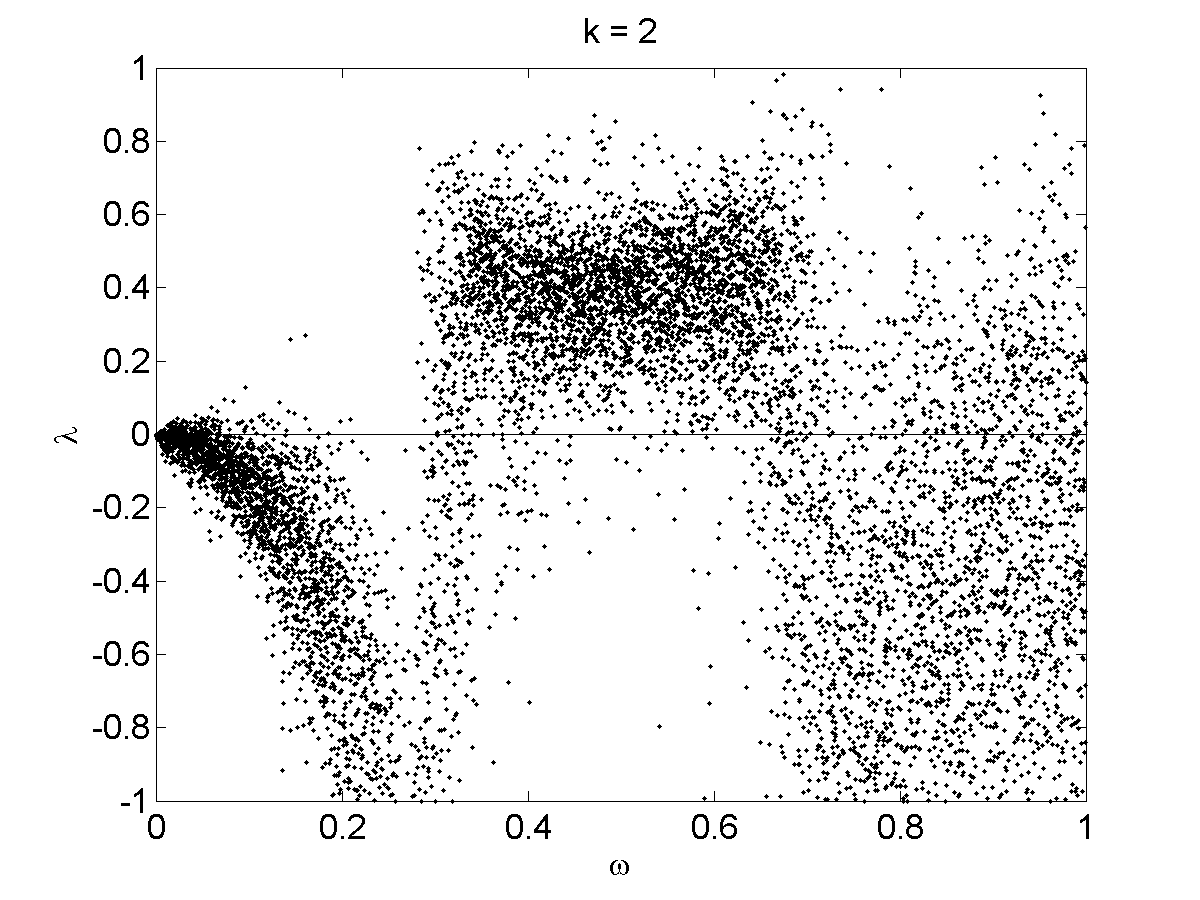
\includegraphics[width=.5\textwidth]{figs/rcirc_u_lyap_10000_L_005_k_2_w.png}\\
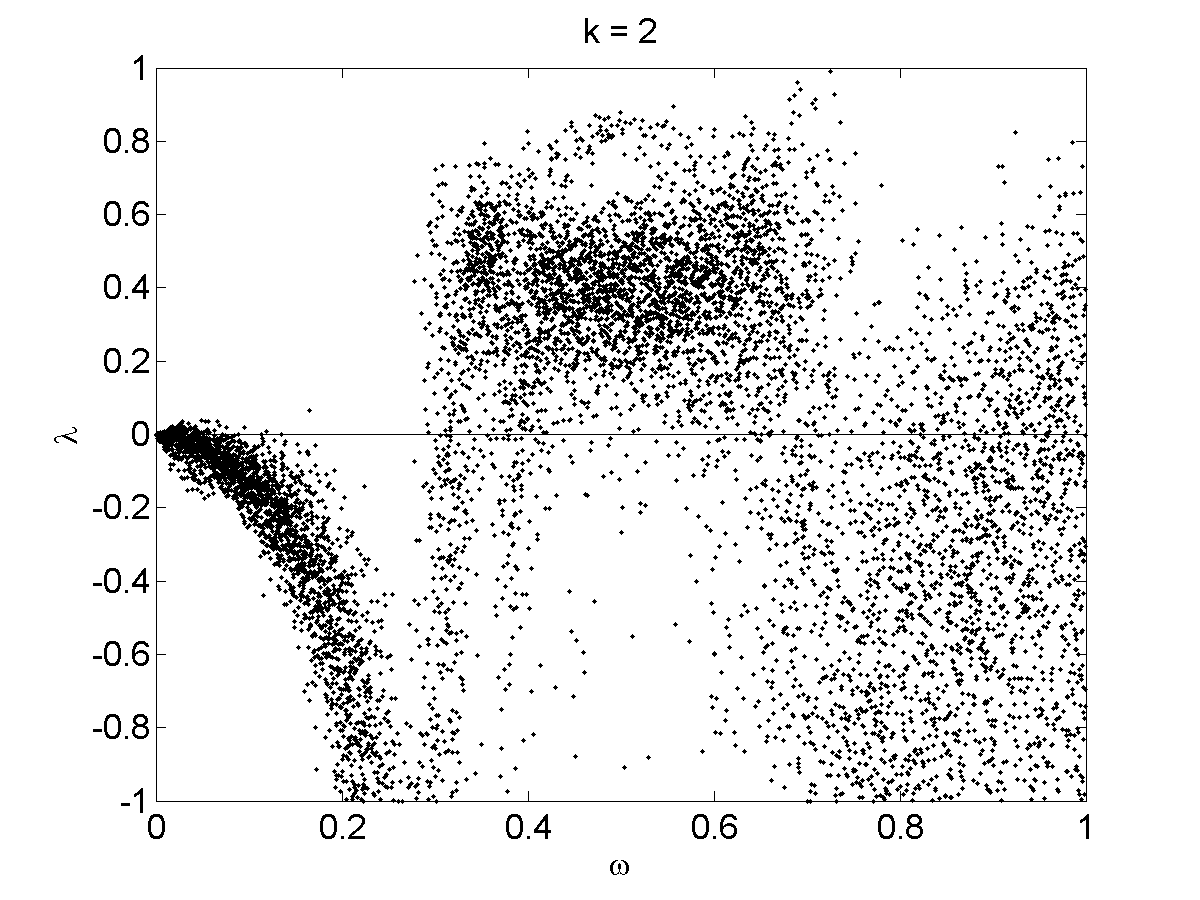
\includegraphics[width=.5\textwidth]{figs/rcirc_u_lyap_10000_L_01_k_2_w.png}\hfill
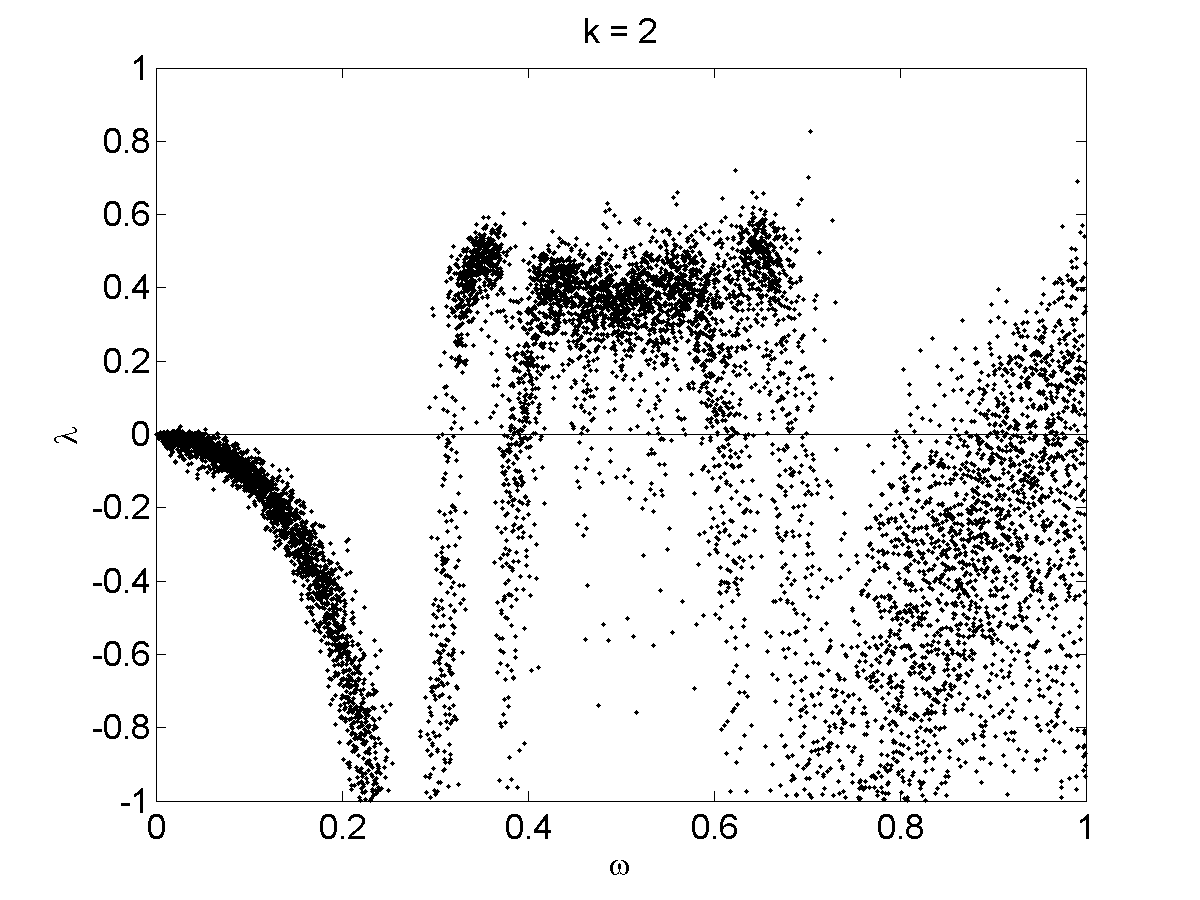
\includegraphics[width=.5\textwidth]{figs/rcirc_u_lyap_10000_L_03_k_2_w.png}\\
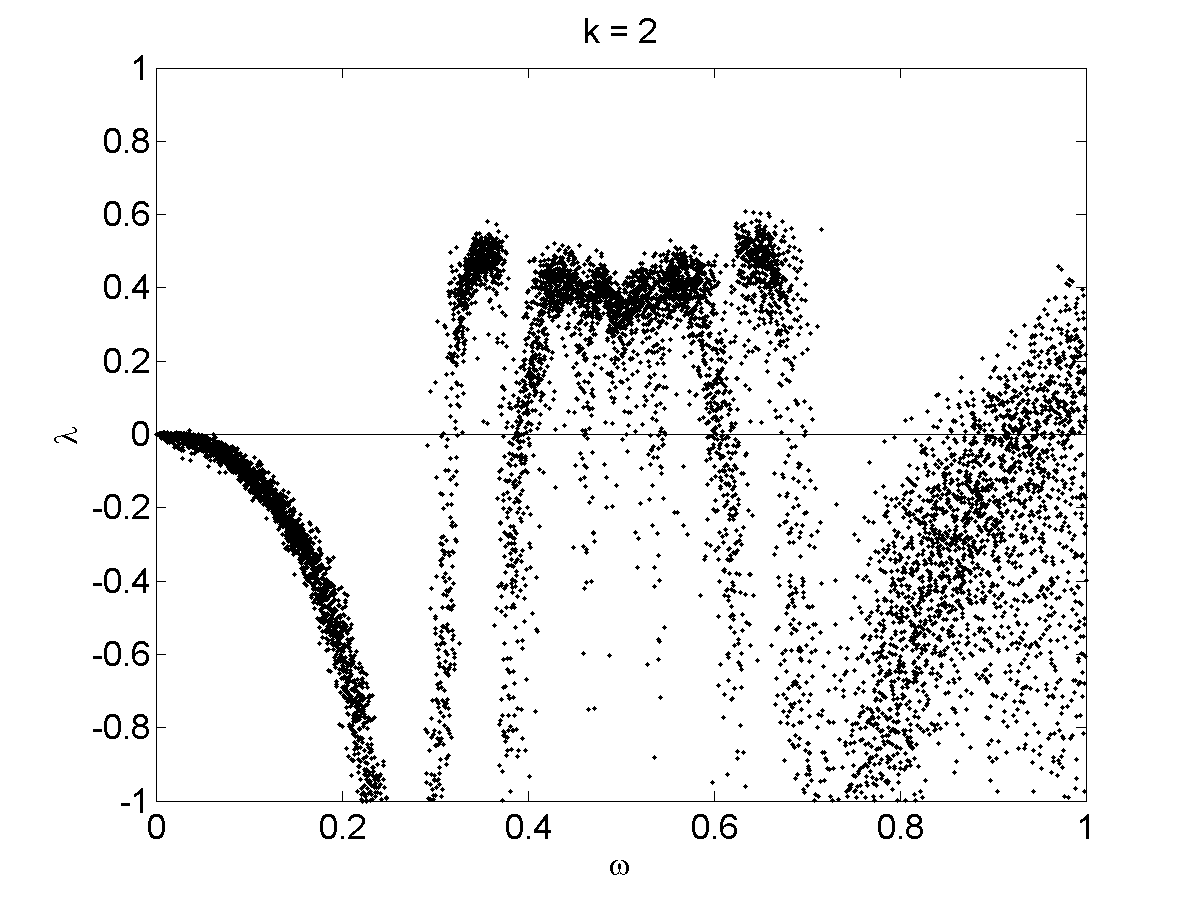
\includegraphics[width=.5\textwidth]{figs/rcirc_u_lyap_10000_L_05_k_2_w.png}\hfill
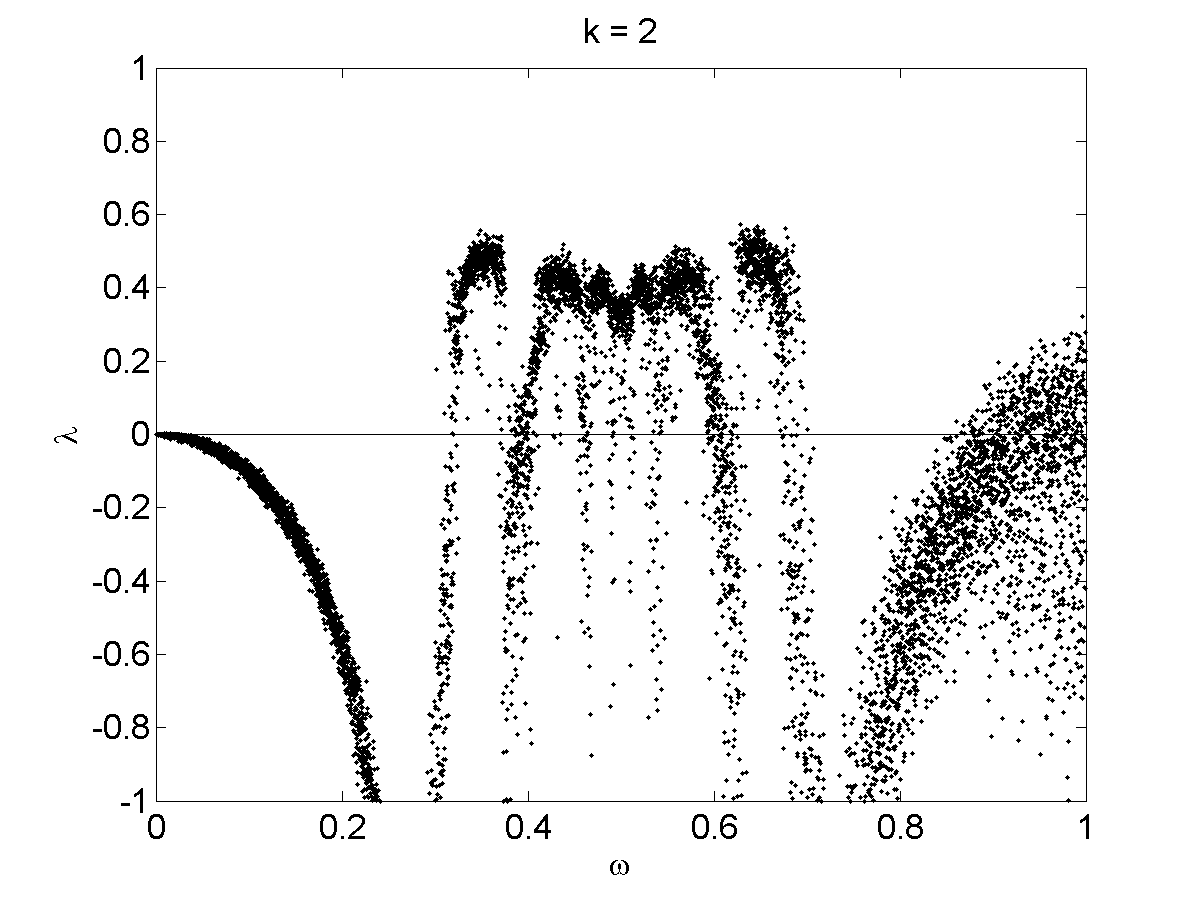
\includegraphics[width=.5\textwidth]{figs/rcirc_u_lyap_10000_L_09_k_2_w.png}\\
\end{figure}

\begin{figure}[!h]
\caption[Lyapunov exponent in the random circle map (uniform distribution) compared to the
deterministic map, varying $k$]{The Lyapunov exponent for the deterministic
  circle map (top left) is compared to the Lyapunov exponent of the random circle map for $L \in \{0.05,0.1,0.3,0.5,0.7\}$, where $x_0=0.7$, $\omega=0.8$,$\alpha = 10^{-5}$, and $\hat{\xi}_n\sim Unif(-M_n,M_n)$ for $k \in [0,5]$. The number of exponents computed was $N_\lambda=10,000$. Plots are read left to right, and top to bottom. }\label{fig:rloglyap2_u}
\centering
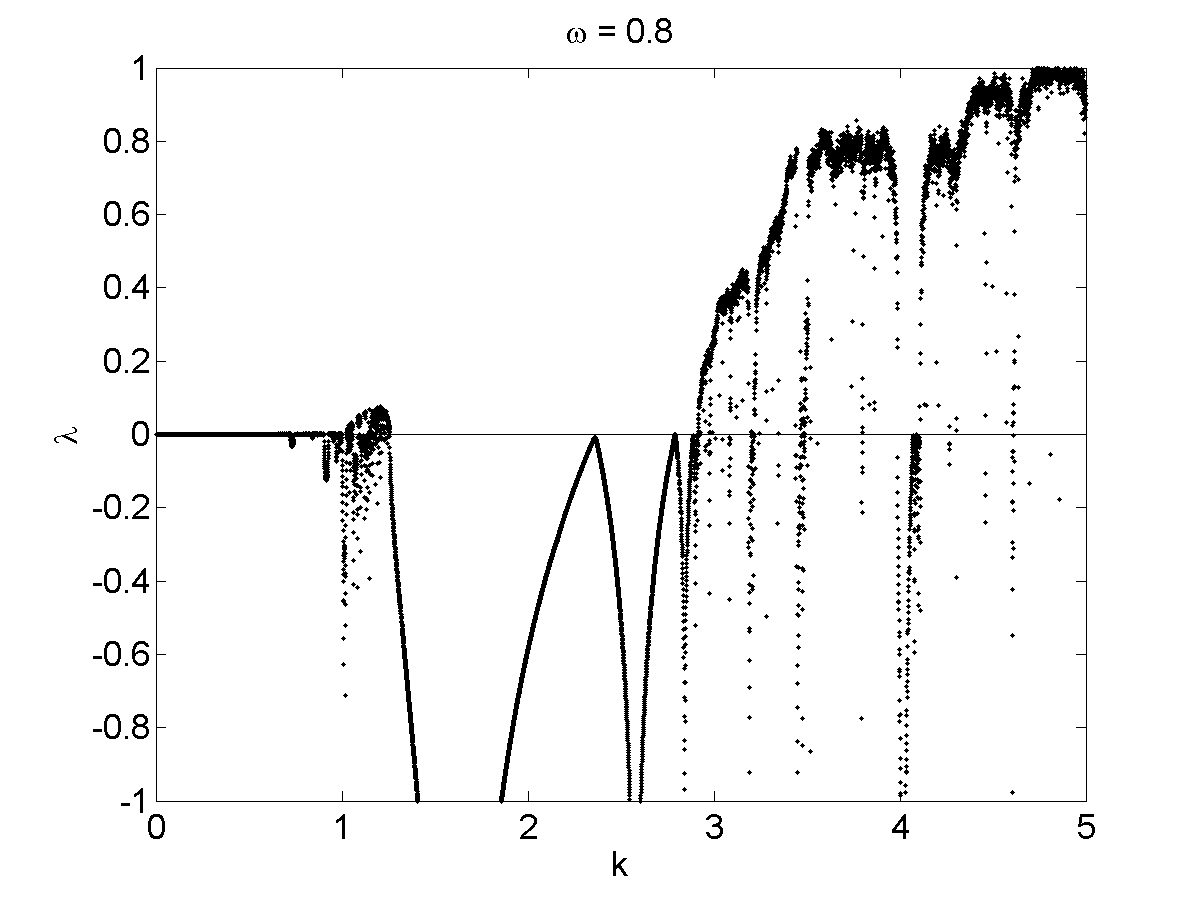
\includegraphics[width=.5\textwidth]{figs/detcirc_n_lyap_10000_w_08_k.png}\hfill
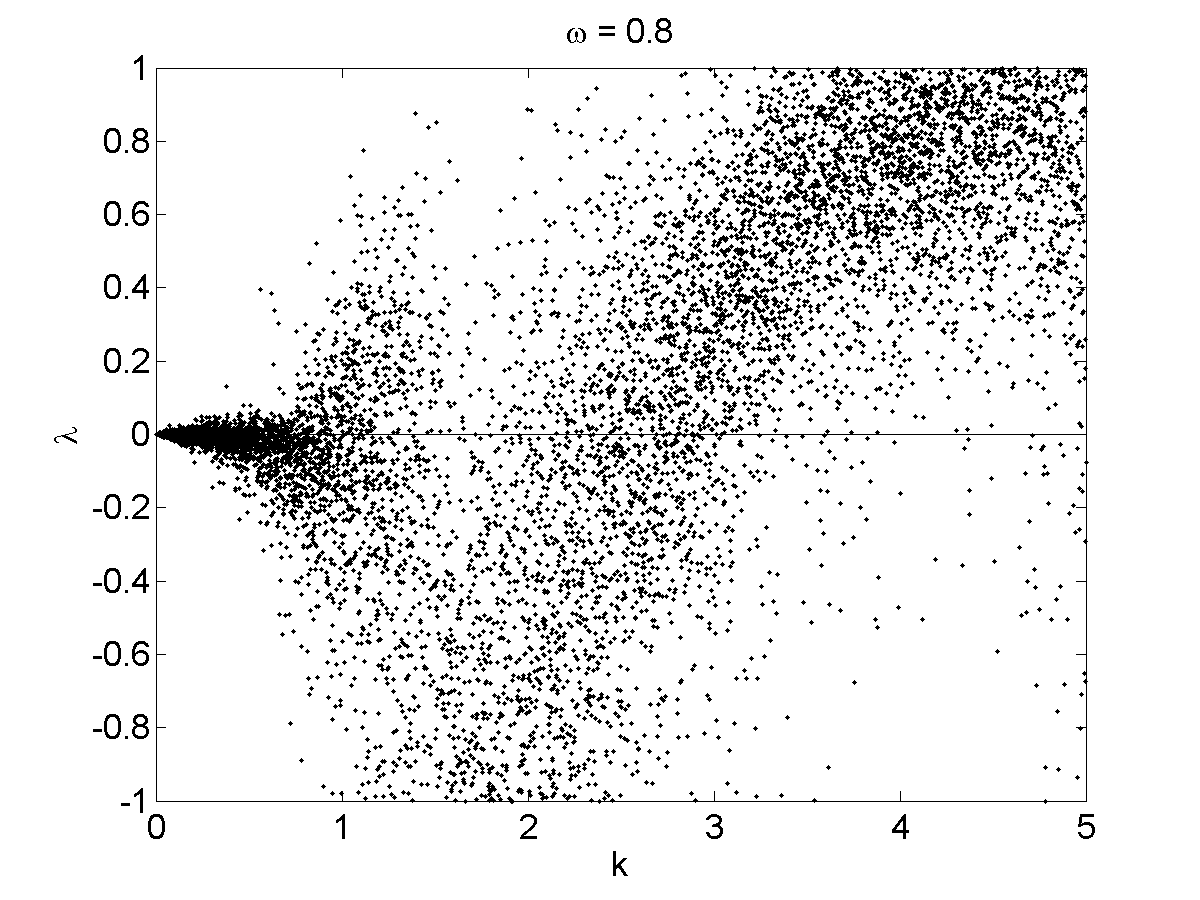
\includegraphics[width=.5\textwidth]{figs/rcirc_u_lyap_10000_L_005_w_08_k.png}\\
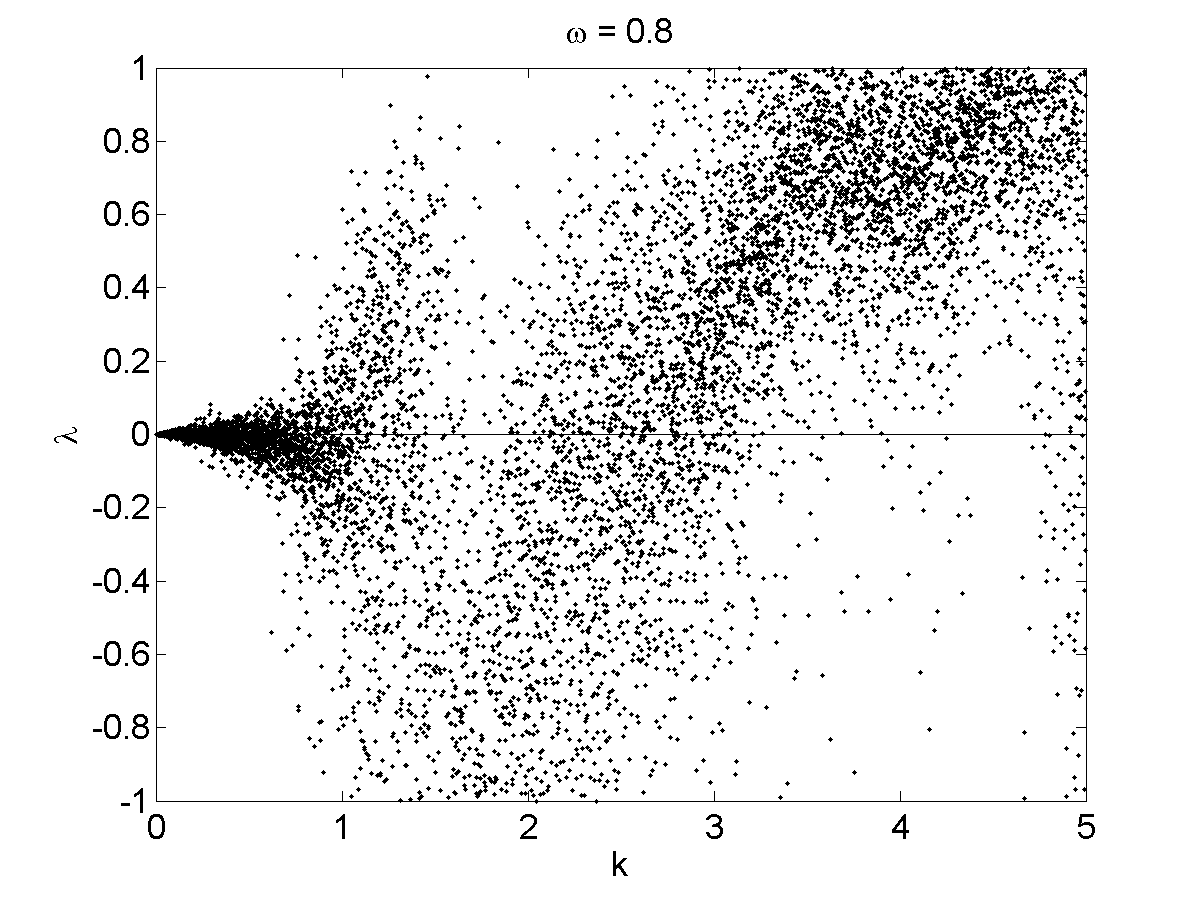
\includegraphics[width=.5\textwidth]{figs/rcirc_u_lyap_10000_L_01_w_08_k.png}\hfill
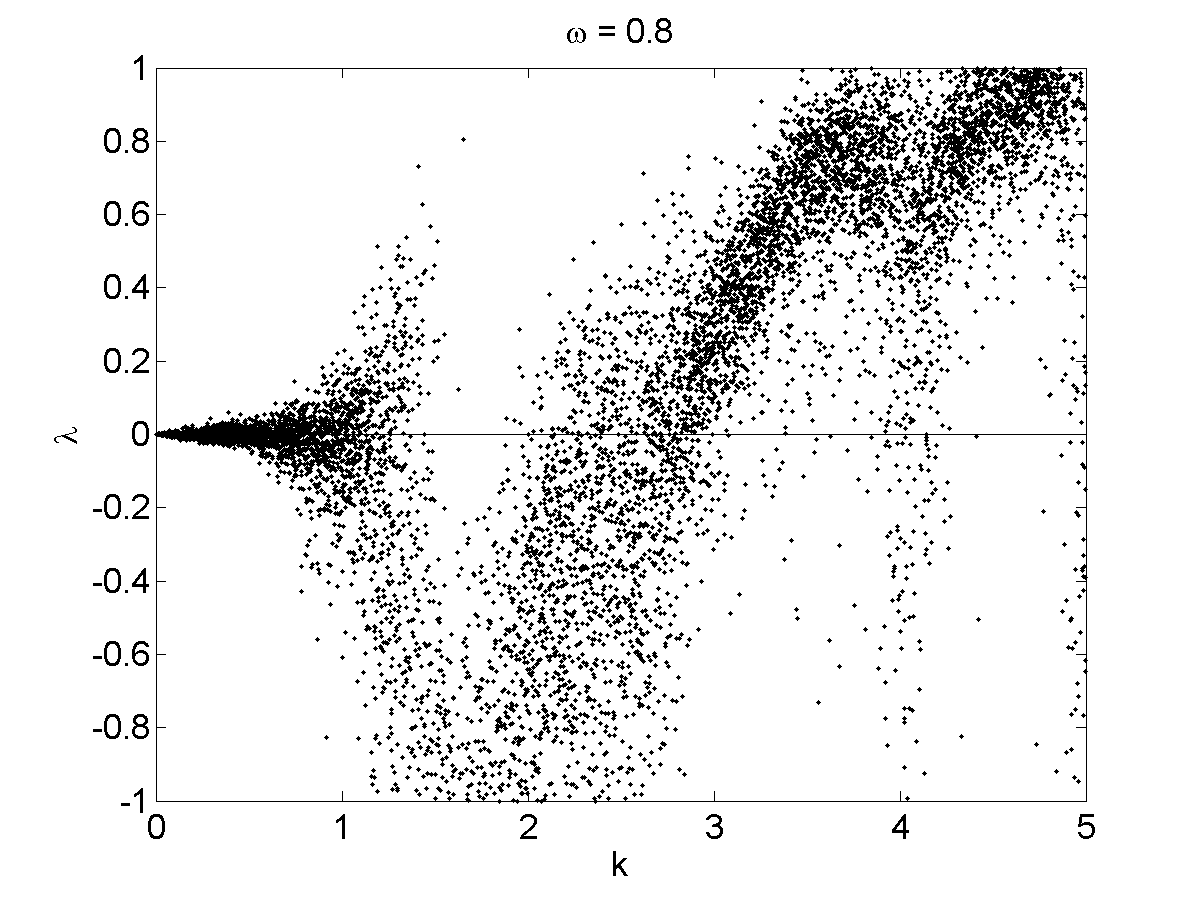
\includegraphics[width=.5\textwidth]{figs/rcirc_u_lyap_10000_L_03_w_08_k.png}\\
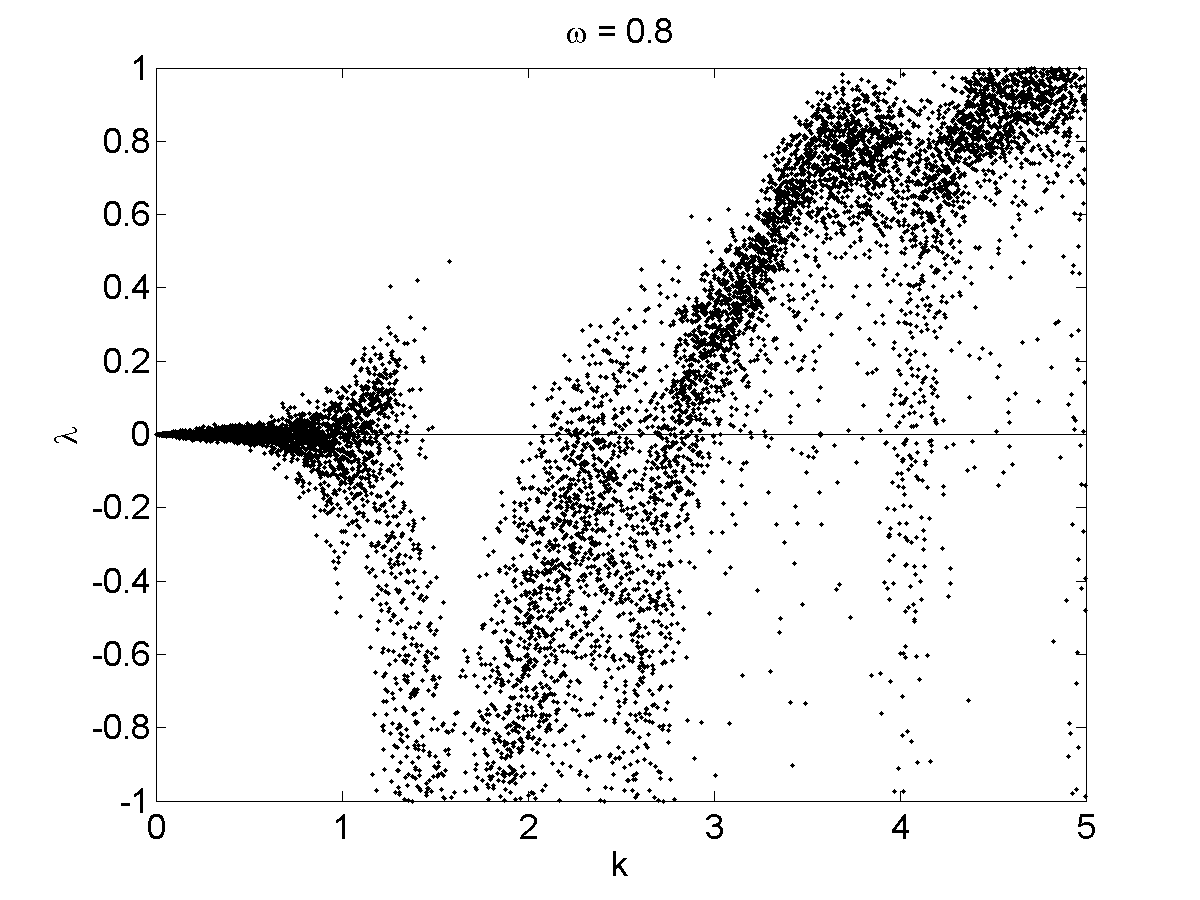
\includegraphics[width=.5\textwidth]{figs/rcirc_u_lyap_10000_L_05_w_08_k.png}\hfill
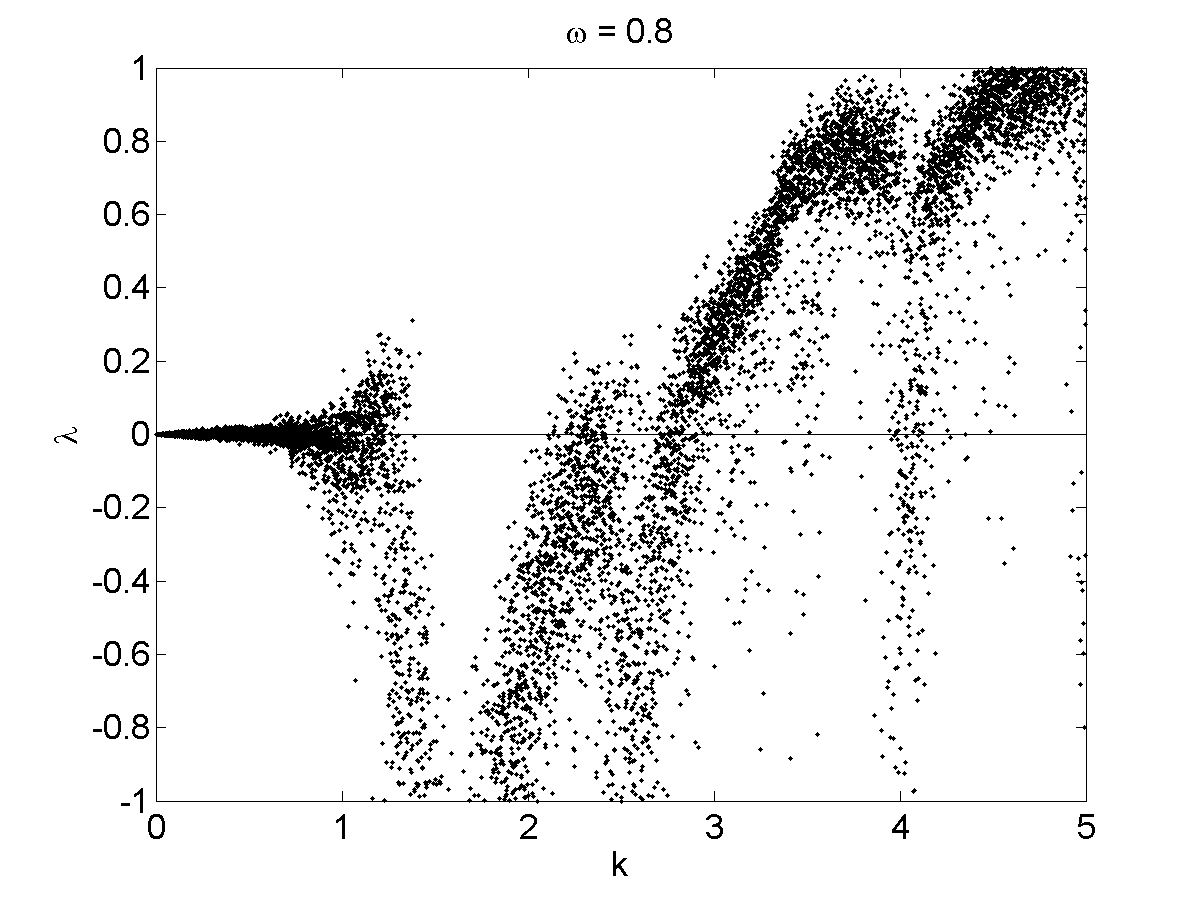
\includegraphics[width=.5\textwidth]{figs/rcirc_u_lyap_10000_L_07_w_08_k.png}\\
\end{figure}

\begin{figure}[H]\linespread{1}
\caption[Average number of period $p$ orbits for the random circle
map]{Average number of period $p$ orbits for the random circle map,
  where $L=0.1$, $\omega =0.1$, $\alpha = 10^{-5}$, $\hat{\xi}_n\sim
  Unif(-M_n,M_n)$ and $k=1$. Results from 1000 simulations of these
  parameters are plotted, using a logarithmic scale for the
  $y$-axis. The error bars indicate the standard error in calculating the mean over 1000 samples.}\label{fig:avgcircorbs}
	\begin{center}
		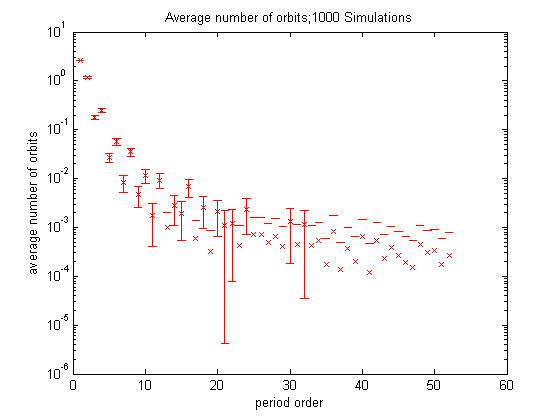
\includegraphics[scale=0.65]{figs/rcirc_avg_num_1000_sim_logscale.png}
	\end{center}
\end{figure}

% \begin{figure}[H]\linespread{1}
% \caption[Bifurcation diagram of the random
% circle map in $(x,\omega)$-space with the uniform distribution]{Bifurcation diagram of the random
% circle map for $L=0.1$, $\omega \in [0,1]$, $\Delta \omega =
% 0.001$,$\alpha = 10^{-5}$, $\hat{\xi}_n\sim Unif(-M_n,M_n)$, 
% and $k=1$. Results from 100 simulations of these parameters are
% plotted. Blue: period 1, red:
% period 2, cyan: period 3, magenta: period 4, green: period 5, black:
% period $p > 5$.} \label{fig:rcirc_bifw_u}
% 	\begin{center}
% 		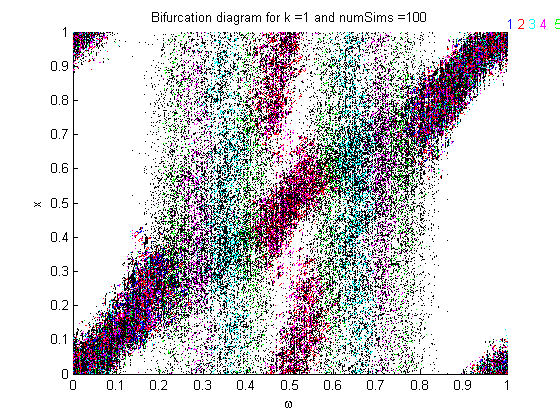
\includegraphics[scale=0.65]{figs/rcirc_bif_L01_k1.png}
% 	\end{center}
% \end{figure}

\begin{figure}[H]\linespread{1}
\caption[The devil's staircase for the random circle map, varying $L$
(uniform distribution)]{The devil's
  staircase for $L=0.05$ (left), $L=0.3$ (middle), and $L=0.5$ (right), where $k=1$,$\alpha = 10^{-5}$ and $\hat{\xi}_n\sim Unif(-M_n,M_n)$. For small $L$, the noise is more pronounced than for large $L$.}\label{fig:randdevil1}
\centering
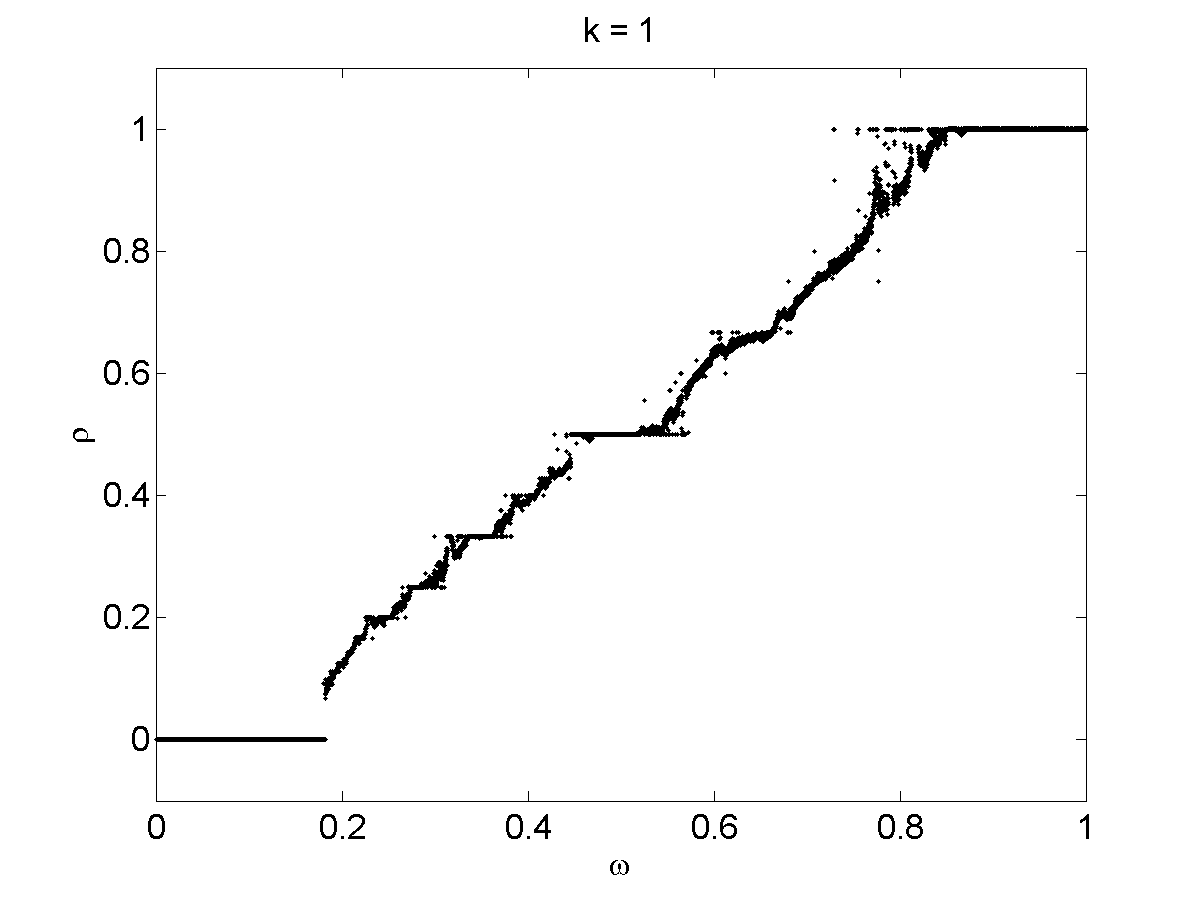
\includegraphics[width=.33\textwidth]{figs/rcirc_u_devil_k1_L005.png}\hfill
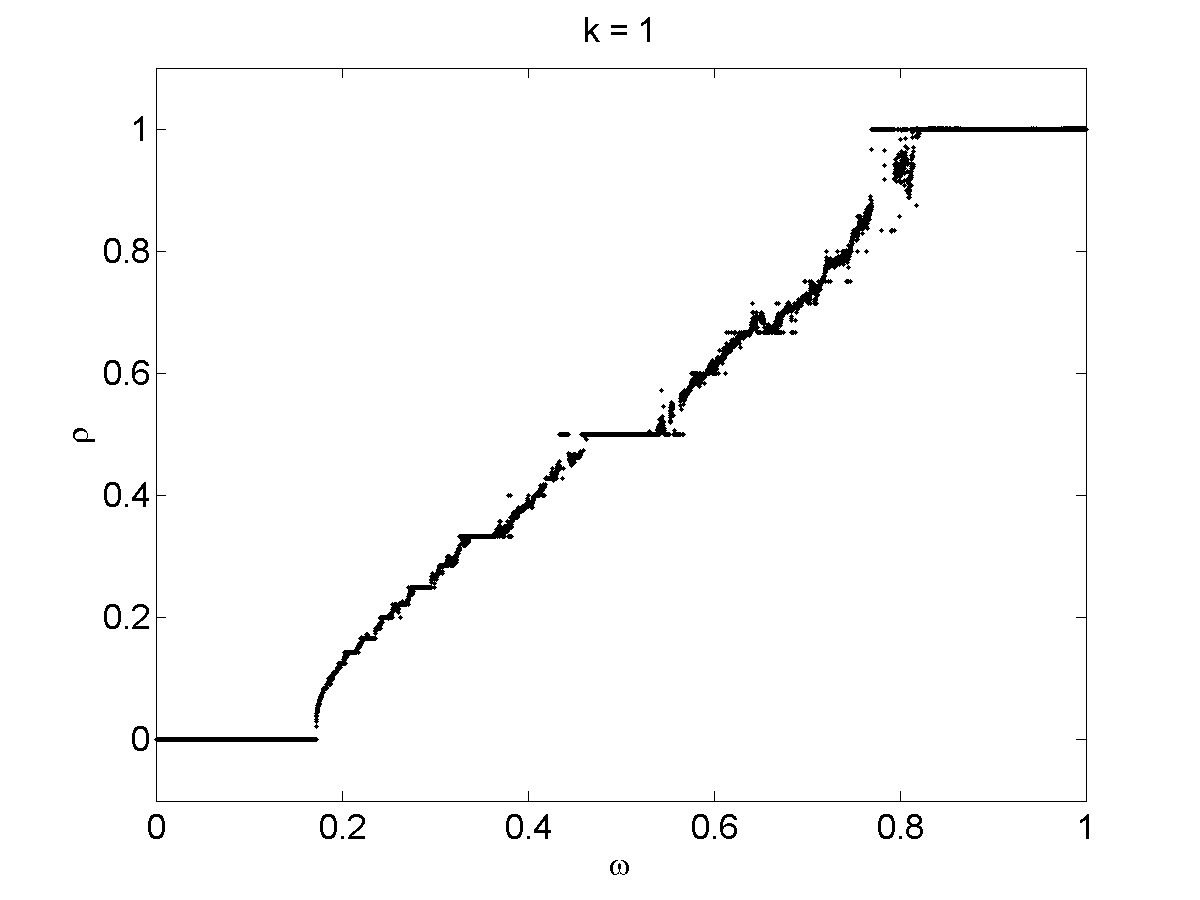
\includegraphics[width=.33\textwidth]{figs/rcirc_u_devil_k1_L01.png}\hfill
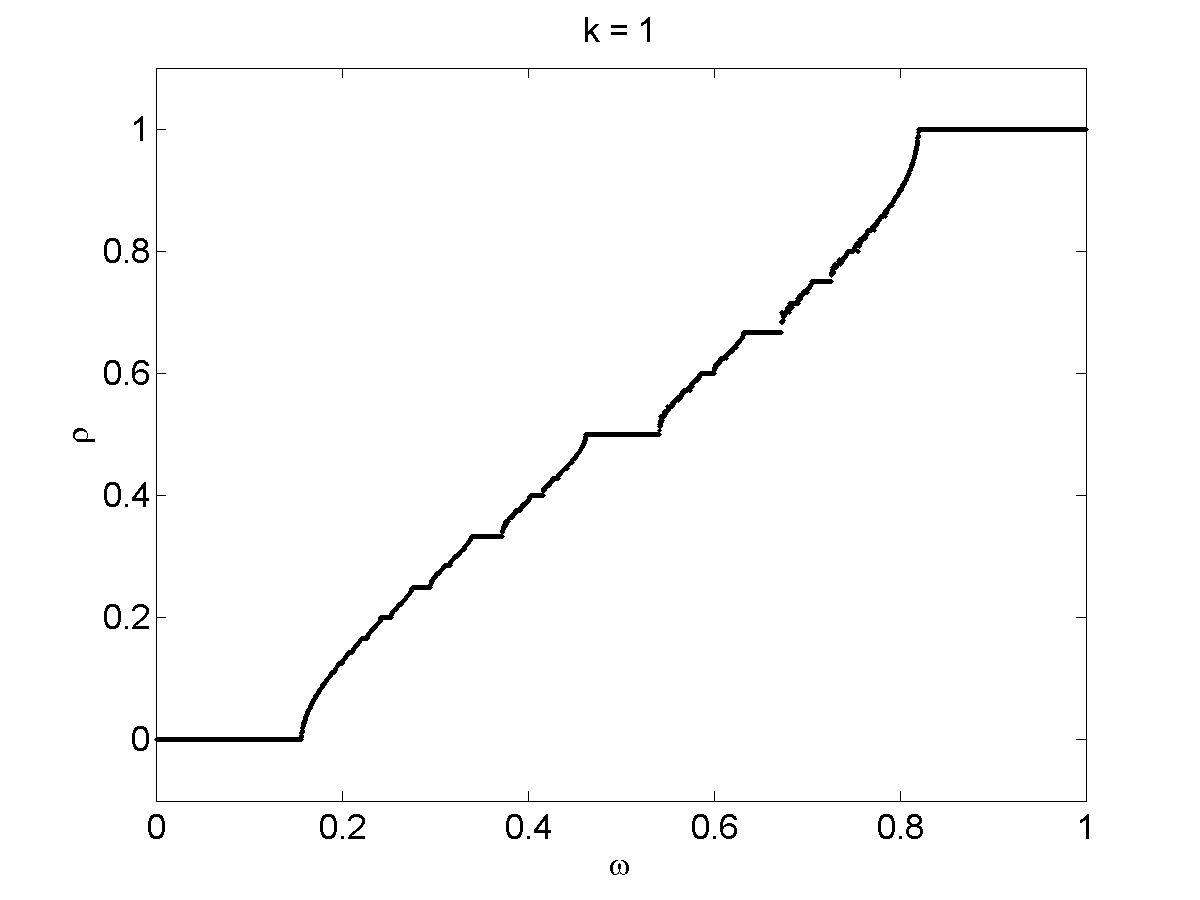
\includegraphics[width=.33\textwidth]{figs/rcirc_u_devil_k1_L05.png}
\end{figure}

\begin{figure}[H]\linespread{1}
\caption[The devil's staircase for the random circle map, varying $k$ (uniform distribution)]{The devil's
  staircase for $k=0.7$ (left), $k=1$ (middle), and $k=1.5$
  (right). In each plot, $\alpha = 10^{-5}$,$\hat{\xi}_n\sim Unif(-M_n,M_n)$ and $L = 0.1$.}\label{fig:randdevil2}
\centering
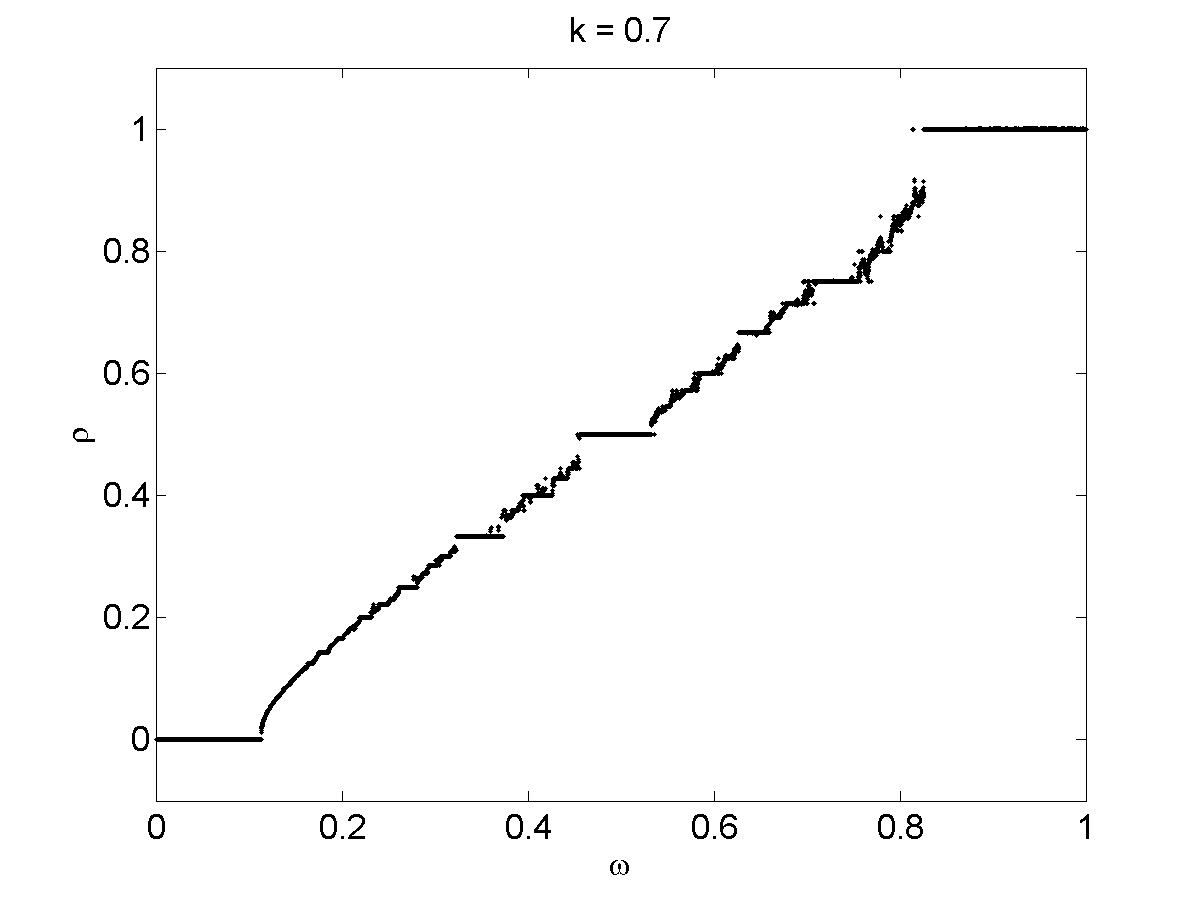
\includegraphics[width=.329\textwidth]{figs/rcirc_u_devil_k07_L01.png}\hfill
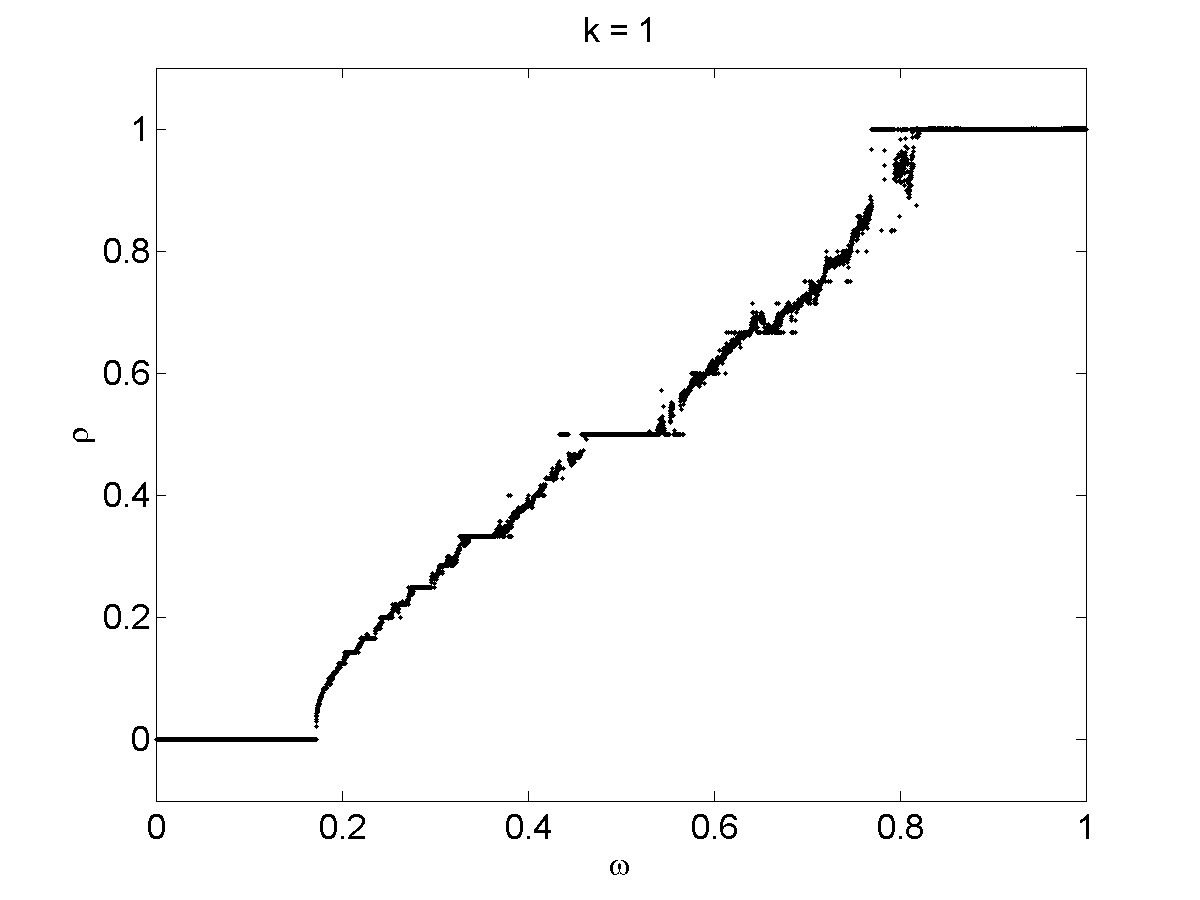
\includegraphics[width=.329\textwidth]{figs/rcirc_u_devil_k1_L01.png}\hfill
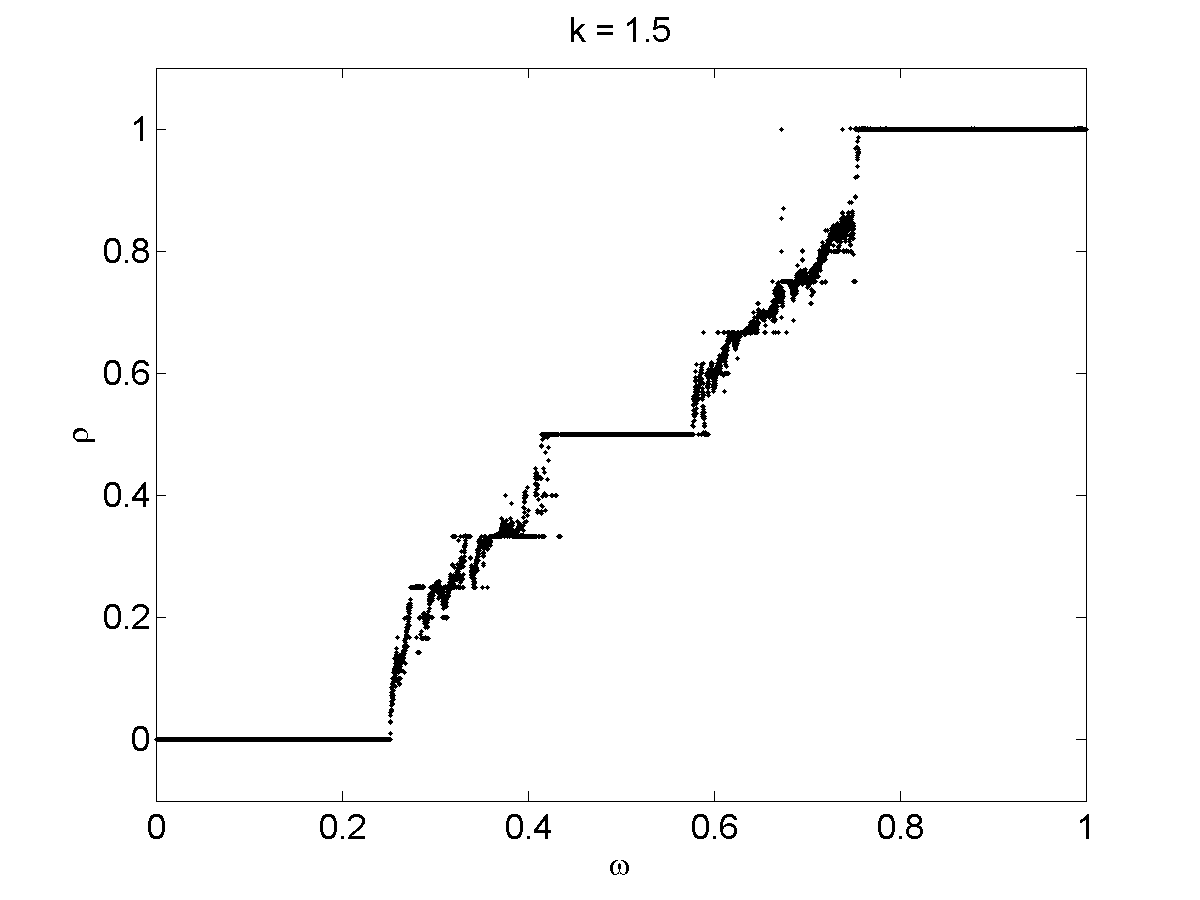
\includegraphics[width=.329\textwidth]{figs/rcirc_u_devil_k15_L01.png}
\end{figure}

% \begin{figure}[H]\linespread{1}
% \caption[Histogram and kernel density estimator of rotation numbers in the random circle
% map]{Histogram of rotation numbers in the random circle map, where
%   $L=0.1$, $k=1$, $\alpha = 10^{-5}$, $\hat{\xi}_n\sim
%   Unif(-M_n,M_n)$, and $\omega = 0.45$. Results from 1000 simulations
%   are plotted.}
% \centering
% 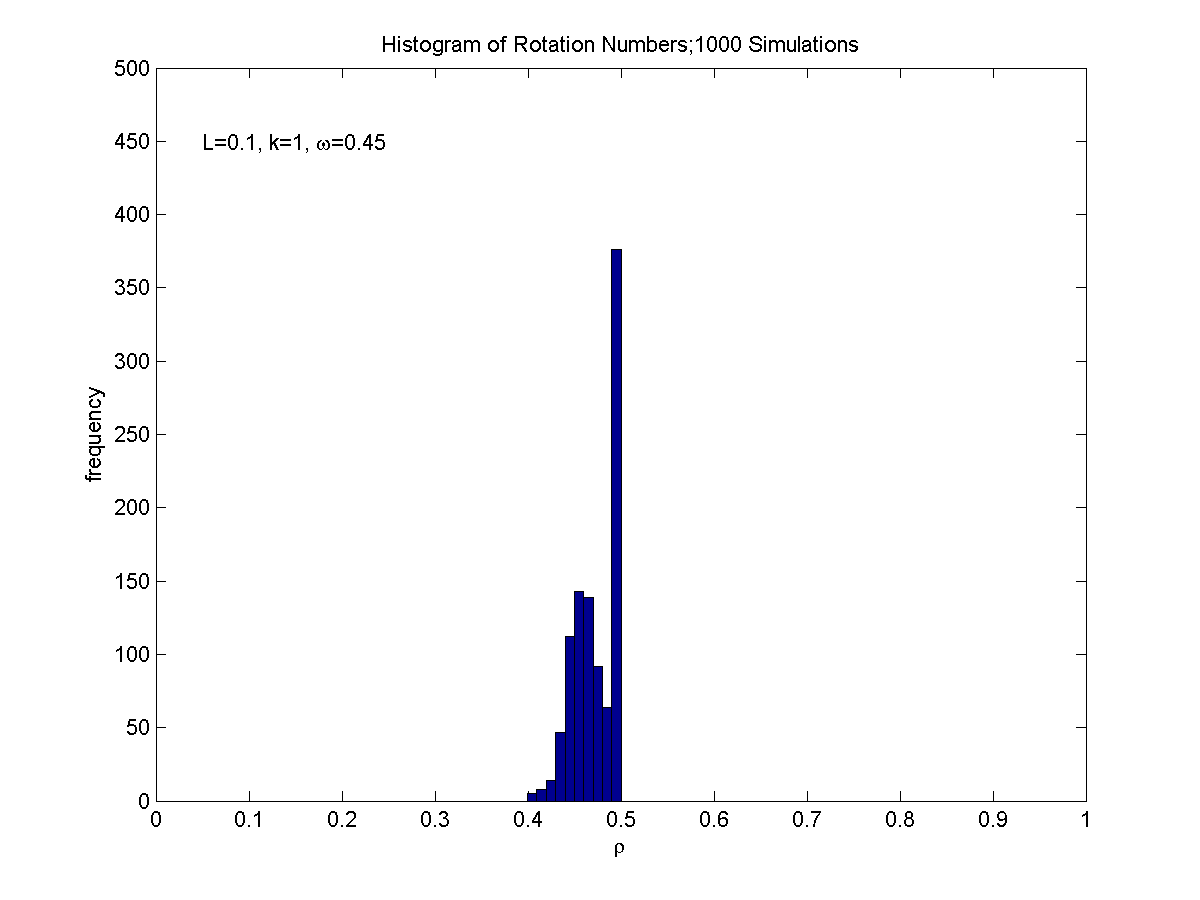
\includegraphics[width=.5\textwidth]{figs/hist_rho_k1_L01_om045.png}\hfill
% 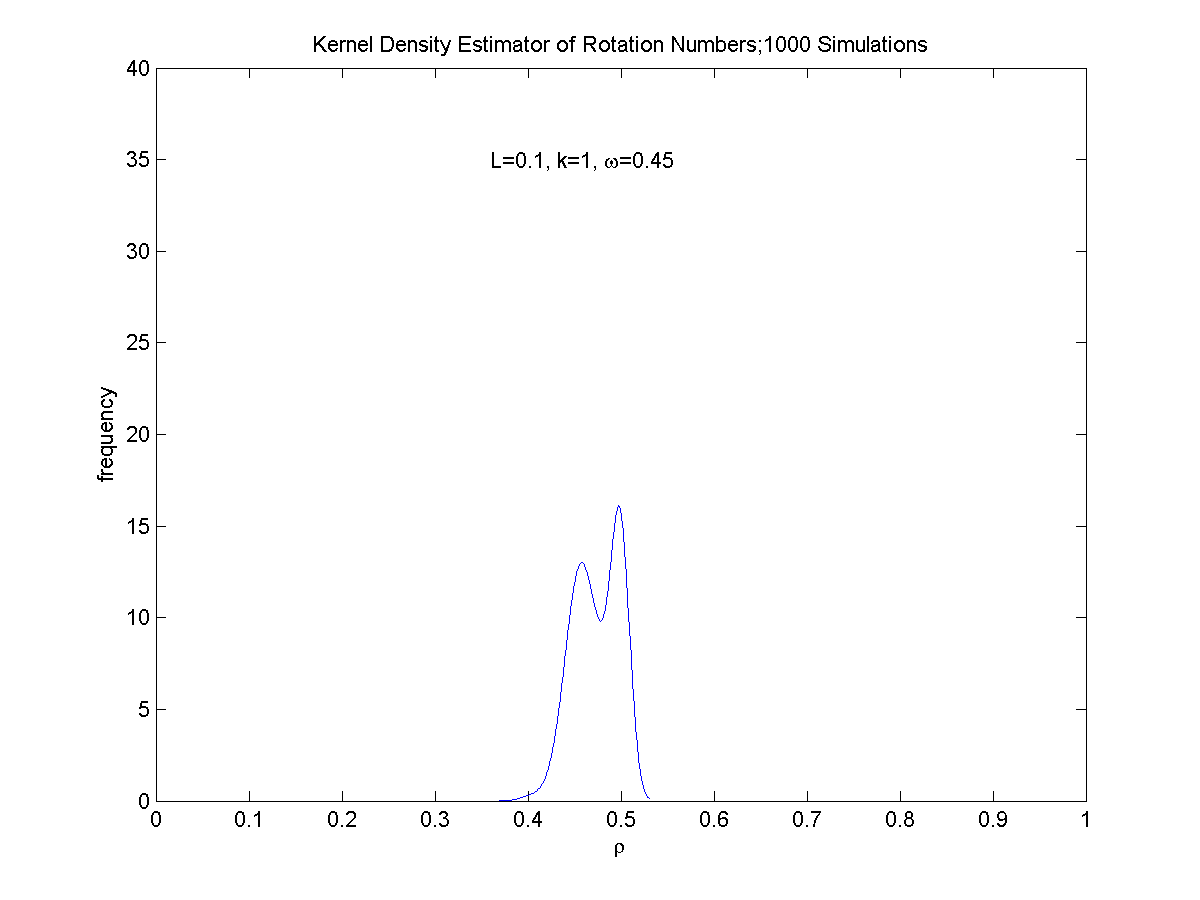
\includegraphics[width=.5\textwidth]{figs/kde_rho_k1_L01_om045.png}
% \end{figure}

\subsection{Normal Distribution}
\begin{figure}[H]\linespread{1}  
\caption[The Arnold tongues for the random circle map, normal distribution]{The Arnold
  tongues for $k\in [0,1.5]$, $\Delta k = 0.0015$, $\omega \in [0,1]$,
  $\Delta \omega = 0.001$, $\alpha = 10^{-5}$, $\hat{\xi}_n\sim
  N(0,\alpha e^{-L|n|})$ and $L_j \in
  \{0.025,0.05,0.1,0.3,0.5,0.9\}$. Plots are ordered left to right, and top to bottom. The colorbar
to the right demonstrates the period and corresponding color.}\label{fig:rcirctongues_n}
\centering
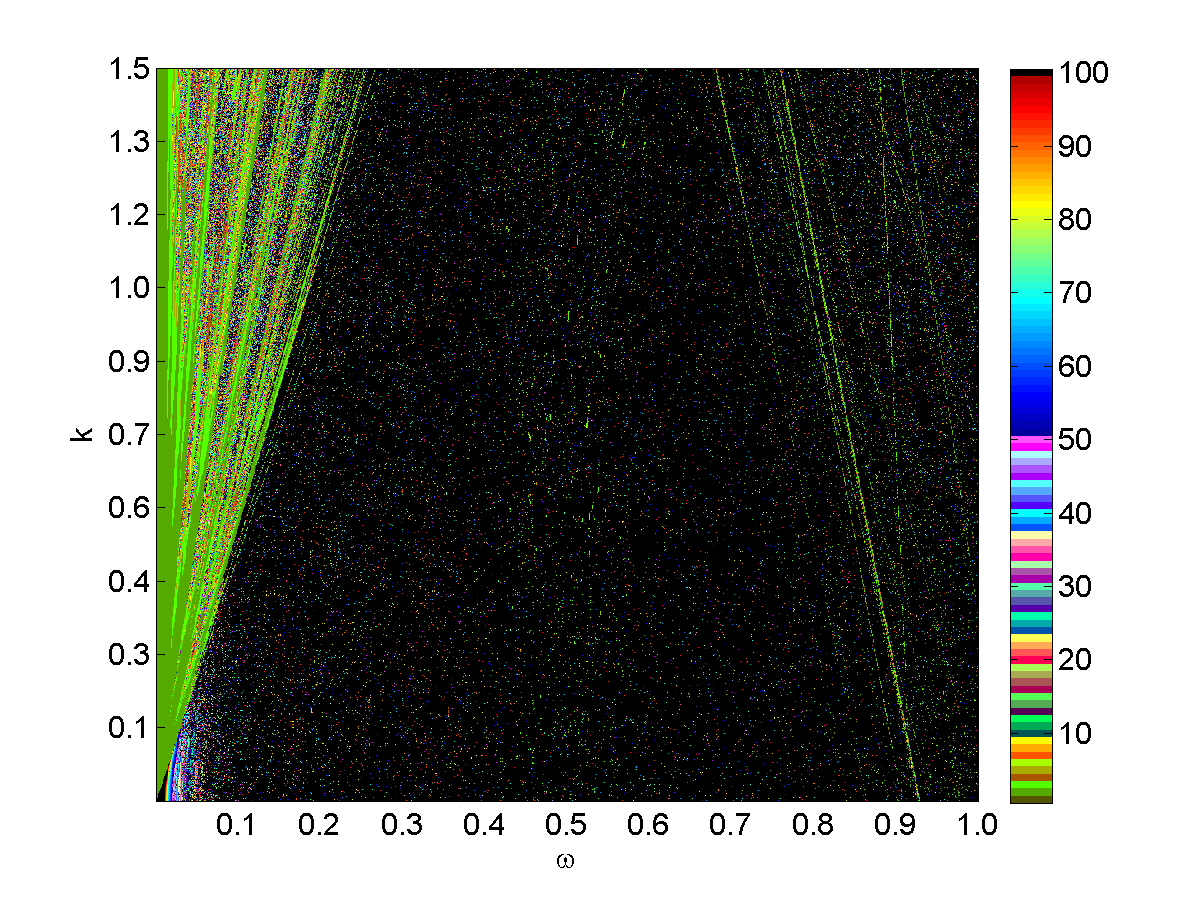
\includegraphics[width=.5\textwidth]{figs/tongues_norm_1000_L_0025.png}\hfill
\includegraphics[width=.5\textwidth]{figs/tongues_norm_1000_L_005.png}\\
\includegraphics[width=.5\textwidth]{figs/tongues_norm_1000_L_01.png}\hfill
\includegraphics[width=.5\textwidth]{figs/tongues_norm_1000_L_03.png}\\
\includegraphics[width=.5\textwidth]{figs/tongues_norm_1000_L_05.png}\hfill
\includegraphics[width=.5\textwidth]{figs/tongues_norm_1000_L_09.png}\\
\end{figure}

\begin{figure}[!h]
\caption[Lyapunov exponent in the random circle map (normal distribution) compared to the
deterministic map, varying $\omega$]{The Lyapunov exponent for the deterministic
  circle map (top left) is compared
  to the Lyapunov exponent of the random circle map for $L \in
  \{0.05,0.1,0.3,0.5,0.9\}$, where $x_0=0.7$, $k=1.5$,$\alpha =
  10^{-5}$, and $\hat{\xi}_n\sim
  N(0,\alpha e^{-L|n|})$ for $\omega \in [0,1]$. The number of exponents computed was $N_\lambda=10,000$. Plots are read left to right, and top to bottom. }\label{fig:rcirclyap_n}
\centering
\includegraphics[width=.5\textwidth]{figs/det_circ_lyap.png}\hfill
\includegraphics[width=.5\textwidth]{figs/rcirc_n_lyap_L_005_w.png}\\
\includegraphics[width=.5\textwidth]{figs/rcirc_n_lyap_L_01_w.png}\hfill
\includegraphics[width=.5\textwidth]{figs/rcirc_n_lyap_L_03_w.png}\\
\includegraphics[width=.5\textwidth]{figs/rcirc_n_lyap_L_05_w.png}\hfill
\includegraphics[width=.5\textwidth]{figs/rcirc_n_lyap_L_09_w.png}\\
\end{figure}

\begin{figure}[!h]
\caption[Lyapunov exponent in the random circle map (normal distribution) compared to the
deterministic map, varying $k$]{The Lyapunov exponent for the deterministic
  circle map (top left) is compared
  to the Lyapunov exponent of the random circle map for $L \in
  \{0.05,0.1,0.3,0.5,0.7\}$, where $x_0=0.7$, $\omega=0.7$,$\alpha =
  10^{-5}$, and $\hat{\xi}_n\sim
  N(0,\alpha e^{-L|n|})$ for $k \in [0,5]$. The number of exponents computed was $N_\lambda=10,000$. Plots are read left to right, and top to bottom. }\label{fig:rloglyap2}
\centering
\includegraphics[width=.5\textwidth]{figs/det_circ_lyap_k.png}\hfill
\includegraphics[width=.5\textwidth]{figs/rcirc_n_lyap_L_005_k_10000.png}\\
\includegraphics[width=.5\textwidth]{figs/rcirc_n_lyap_L_01_k_10000.png}\hfill
\includegraphics[width=.5\textwidth]{figs/rcirc_n_lyap_L_03_k_10000.png}\\
\includegraphics[width=.5\textwidth]{figs/rcirc_n_lyap_L_05_k_10000.png}\hfill
\includegraphics[width=.5\textwidth]{figs/rcirc_n_lyap_L_07_k_10000.png}\\
\end{figure}

\begin{figure}[H]\linespread{1}
\caption[The devil's staircase for the random circle map, varying $L$
(normal distribution)]{The devil's
  staircase for $L=0.05$ (left), $L=0.3$ (middle), and $L=0.5$ (right), where $k=1$,$\alpha = 10^{-5}$ and $\hat{\xi}_n\sim N(0,\alpha e^{-L|n|})$. For small $L$, the noise is more pronounced than for large $L$.}\label{fig:randdevil1_n}
\centering
\includegraphics[width=.33\textwidth]{figs/rcirc_n_devil_k1_L005.png}\hfill
\includegraphics[width=.33\textwidth]{figs/rcirc_n_devil_k1_L03.png}\hfill
\includegraphics[width=.33\textwidth]{figs/rcirc_n_devil_k1_L05.png}
\end{figure}

\begin{figure}[H]\linespread{1}
\caption[The devil's staircase for the random circle map, varying $k$ (normal distribution)]{The devil's
  staircase for $k=0.7$ (left), $k=1$ (middle), and $k=1.5$
  (right). In each plot, $\alpha = 10^{-5}$,$\hat{\xi}_n\sim
  N(0,\alpha e^{-L|n|})$ and $L = 0.1$. The discontinuities increase as
$k$ grows.}\label{fig:randdevil2_n}
\centering
\includegraphics[width=.33\textwidth]{figs/rcirc_n_devil_k07_L01.png}\hfill
\includegraphics[width=.33\textwidth]{figs/rcirc_n_devil_k1_L01.png}\hfill
\includegraphics[width=.33\textwidth]{figs/rcirc_n_devil_k15_L01.png}
\end{figure}
